% !TeX encoding = utf-8
% !TeX program = xelatex

% !Mode:: "TeX:UTF-8"
%%  正式稿使用 XeLaTeX 加载 Times New Roman 正文字体。

%%  注意：
%%   1. 文件默认的编码为 UTF-8 对于windows，请选用支持UTF-8编码的编辑器。
%%   2. 若是模板有什么问题，请及时与我们取得联系，Email：latexstudio@qq.com。
%% 开箱即用的模版链接： https://www.texhub.com/templates/6aeebe53ea83bc86214917f9

\PassOptionsToPackage{hypertexnames=false}{hyperref}
\documentclass{swmcmthesis}
\ifxetex
    \usepackage[no-math]{fontspec}
    % 等 newtxtext 设置完字体后加载 Times New Roman，保留现有数学符号字体。
    \AtEndPreamble{%
        \defaultfontfeatures{Ligatures=TeX}%
        \setmainfont{Times New Roman}%
    }
    \setlength{\emergencystretch}{1.5em}
\fi
\captionsetup[figure]{
labelfont={bf},
name={Fig.}, 
labelsep=period 
}
%%%%%%%%%%%%填写相关信息%%%%%%%%%%%%%%%%%%%%%%%%%%
\title{Rapid UAV Localization via Coordinated Mobile Vehicles} %论文题目

\baominghao{SWBMCM2619567}           %报名号，修改为自己的队号

\zubie{B} %选题

% 英文摘要由队员确认讨论稿，OpenCode（Magpie，group/gpt-6.2-sol）辅助拟订和核对，供 AI 使用报告记录。
\abstract{%
Coarse alerts provide approximate locations for unmanned aerial vehicles (UAVs).
To refine each horizontal estimate by bearing intersection, two ground vehicles must observe simultaneously.
This study links station selection to vehicle scheduling, quantifies pointing reliability after travel, and compares two rescheduling strategies under disturbances.

For Question one, vehicle geometry, unobstructed three-dimensional lines of sight, and gimbal elevation limits define the observable region for \(T_1\).
The \(80^\circ\) elevation limit gives an attainable minimum horizontal distance of 7.582~m, yielding a maximum observation quality of \(0.13189\,\mathrm{m}^{-1}\) for \(Q=1/r\).
Among the tied stations, \(V_4\) reaches \((91.156,66.121)\)~m with the shortest feasible drive of 3.673~m.

For Question two, the west--north station pair for \(V_3\) and \(V_5\) gives a \(90^\circ\) bearing intersection at the shortest permitted ranges to \(T_2\) and attains the minimum first-order horizontal root mean square error (RMSE) of 0.143623~m.
Rounding a second, clearance-binding pair to millimeters after adding elevation margin gives an RMSE of 0.146102~m, with both driving times below 30~s.
For concurrent alerts, a branch-and-bound search assigns \(V_3\) to \(T_1\) and then \(T_3\), allowing a separate pair to prepare for \(T_2\) in parallel.
Under the same constraints, the millimeter-coordinate schedule advances the latest observation start time from 10.969~s under the nearest-assignment heuristic to 10.392~s.

For Question three, projected-normal integration gives cumulative travel limits for staying within a \(5^\circ\) bearing tolerance with at least 95\% probability.
At a horizontal target distance of 40~m, the limits are 73.936~m for the commanded bearing and 66.837~m for actual pointing with gimbal errors.
At 80~m of travel, the corresponding upper bounds on the per-axis localization standard deviation \(a+80b\) round to 1.779~m and 1.637~m.

For Question four, Field-Wide Rescheduling (FW) and strict retention (SR) use the same millimeter-coordinate initial plan.
FW starts every alert in all 1,751 main-rule scenarios, and SR does so in 7.
The mean latest-start scores, including the 60~s penalty for missed starts, are 24.746~s for FW and 59.802~s for SR.
Across 1,314 matched outage scenarios, deferring later departures and new joint starts until recovery raises the FW mean from 26.436 to 32.301~s.
Under each rule, FW starts every alert in all 1,314 scenarios and records every alert for an uninterrupted five seconds in 876.
}

\keywords{Observable region, bearing intersection, pointing reliability, vehicle scheduling}

\date{2026}

\begin{document}

% 生成首页
\maketitle
% 目录
{\linespread{1.16}\selectfont
\value{tocdepth}=2\relax % 目录仅显示到二级
\tableofcontents
\par}

\newpage

% -------------------------正文开始
\setcounter{page}{1}
% 此行距用于正文及参考文献，给图表和后续段落留出同页排版空间。
\begingroup
\linespread{1.24}\selectfont
% 页顶和页底图表与正文之间留出约一行，避免为浮动体额外断页。
\setlength{\textfloatsep}{12pt plus 2pt minus 2pt}
\section{Introduction}



\subsection{Background}
% \lipsum[1-2]
During the operation of low-altitude airspace monitoring and control, the detection and localization of small Unmanned Aerial Vehicles (UAVs) are a common and challenging problem. Existing reconnaissance systems can only provide coarse alert information containing an approximate azimuth, horizontal distance, and altitude, and such information cannot yield the precise geolocation of the target; failure to locate the target in time will weaken low-altitude airspace security and increase the risk of intrusion into restricted areas. Therefore, developing efficient rapid direction-finding and localization technology is of great significance for the stable and reliable operation of low-altitude monitoring systems. In two-station bearing-only localization, the intersection of two nonparallel bearing lines estimates the target's horizontal position. The sensor-to-target geometry governs how bearing errors affect localization accuracy~\cite{ref:bearing-geometry}. Based on this strategy, and according to the preset field layout, building data, and initial vehicle positions, initial conditions are provided for the design and evaluation of subsequent observation-station selection, vehicle assignment and routing, and rescheduling strategies.
\subsection{Work}
% \lipsum[1-2]
Taking the five standby observation vehicles and the three base alerts within the square operational field as the research object, this study focuses on rapid UAV localization via coordinated mobile vehicles, based on the field layout, building data, initial vehicle positions, and alert parameters provided in the problem, with the core goal of achieving high-accuracy intersection localization and efficient vehicle assignment under observability, timing, and geometric constraints. The following four problems need to be solved:

\textbf{Problem 1}: Determine the vehicle-observable region for target \textbf{T1} and illustrate the result with a plot, where a station is observable only when the vehicle geometric constraints, line-of-sight(LOS) occlusion constraints, and feasible gimbal elevation bounds are satisfied concurrently. Adopting $Q = 1/r$ as the observation-quality metric, locate the optimal observation station, report its horizontal distance to the target and LOS elevation angle, explicitly state the mathematical optimization criterion for "optimal," and specify reasonable tie-breaking rules when multiple stations attain the same optimal value.

\textbf{Problem 2}: \textbf{(1)} For two-station intersection localization, construct a mathematical model that relates localization accuracy to geometric station parameters, including baseline length, intersection angle, and target range; define an accuracy metric and justify its rationality. Under the constraint that the travel time from each vehicle's initial position to its assigned station does not exceed 30 s, select two vehicles from the five available and determine the optimal station pair for alert \textbf{T2}; report the station coordinates, baseline length, intersection angle, vehicle travel times, and resulting accuracy metric, and discuss whether the model degenerates as the intersection angle approaches $0^\circ$ or $180^\circ$ or when stations lie on the observable-region boundary, proposing corresponding handling strategies. \textbf{(2)} For the three alerts \textbf{T1}, \textbf{T2}, and \textbf{T3} released simultaneously at $t = 0$, design a vehicle assignment and routing scheme that minimizes the maximum observation start time, and output the complete timeline of each vehicle marking departure, arrival at the station, gimbal slew, observation start and end, gimbal reset, and subsequent departure; separately define a nearest-assignment heuristic, solve a baseline scheme under the same constraints, and compare it with the optimized scheme to analyze the sources of the differences.

\textbf{Problem 3}: Considering the random errors in vehicle localization and gimbal pointing control, construct an error propagation model for the bearing deviation $\Delta\psi$. Determine the maximum allowable travel distance such that $P(|\Delta\psi| \leq 5^\circ) \geq 0.95$; if the same accuracy requirement must still hold when the vehicle travels 80 m, derive the constraints on the nonnegative parameters $a$ and $b$ in the localization standard-deviation model $\sigma(s) = a + bs$. Justify the applicability of any approximations or numerical methods used in the modeling, validate the results, compare the relative contributions of the three error sources to the horizontal bearing deviation, and provide practical deployment insights.

\textbf{Problem 4}: Taking the scheduling solution obtained in \textbf{Problem 2(2)} as the baseline, consider the disturbances and their combinations occurring at $t = 5 s$: a new alert requiring two observation vehicles, the random failure of exactly one vehicle, and a communication outage. Develop a rescheduling model and compare its performance against the policy of retaining the original schedule, presenting results for both single disturbances and combined disturbances. Using the completion ratio $\eta = \frac{K}{N}$ and the latest observation start time \(t_{\mathrm{last}}\) as evaluation metrics over the window $t \in [0, 60] s$, report \((\eta,t_{\mathrm{last}})\), the rescheduling policies, and the vehicle timelines for each scenario; analyze the scenarios where rescheduling yields benefits and where it performs poorly, and explain the underlying causes.


\section{Problem analysis}
\subsection{Analysis of Problem one}
The core of Problem 1 is to establish a vehicle-observable region model under three types of constraints—vehicle geometric, LOS occlusion, and gimbal elevation bounds—and complete the optimal-station analysis under the observation-quality metric \(Q=1/r\).

To construct the feasible region, each observation vehicle is first modeled as a disk of equivalent radius \(1.5\) m, and the field boundary together with the building footprints is converted into center-point clearance constraints. The three-dimensional sight segment from the camera to the target is then checked against every building prism, where any intersection, tangency, or contact is counted as occlusion; this judgment is equivalently represented by shadow polygons on the camera-height plane. Combined with the elevation bound that relates the sight-line angle to the horizontal distance, the intersection of these feasible sets yields the observable region, which is illustrated by a scientific plot.

On this basis, the observation quality \(Q=1/r\) is adopted as the optimization metric, so maximizing Q is equivalent to finding the feasible point closest to the target's horizontal projection. The elevation constraint analytically gives the lower bound of the horizontal distance, and verifying that a feasible station exists on this bound circle establishes the continuous global optimum. For the equally optimal stations lying on the resulting optimal arc, we consider two secondary optimization criteria to determine a practically suitable deployment station. They are respectively the Minimum Travel Distance Criterion and the Maximum Minimum Clearance Criterion.


\subsection{Analysis of Problem two}
Problem 2 investigates two closely related problems: two-station localization accuracy optimization and multi-target observation scheduling with limited vehicle resources.

For Problem 2(1), two observation vehicles are required to synchronously measure the horizontal position of target \textbf{T2}. Since the measurements contain independent random errors, the intersection of the two bearing lines deviates from the actual target position. The localization accuracy is affected by several geometric factors, including the distances between the two observation stations, as well as the intersection angle of the two bearing lines. In addition, the observation stations must satisfy the vehicle accessibility, LOS visibility, gimbal elevation, and vehicle travel-time constraints. Therefore, the first task is to establish an error propagation model and optimize the observation geometry under the operational constraints.

For Problem 2(2), three alerts \textbf{T1}, \textbf{T2}, and \textbf{T3} arrive simultaneously, and each requires two vehicles for synchronous observation. However, only five observation vehicles are available, making vehicle reuse unavoidable. Unlike Problem 2(1), which focuses primarily on localization accuracy, this problem emphasizes the coordination of vehicle assignments, station selection, and observation sequences. In particular, the time required for vehicle movement, gimbal slewing, synchronized observation, and gimbal resetting must all be incorporated into the scheduling process. The objective is to minimize the latest observation start time among the three alerts.

Accordingly, we develop a geometric error propagation model for Problem 2(1) and a continuous-space, event-based vehicle scheduling model for Problem 2(2). The former determines the optimal observation geometry, while the latter seeks an efficient multi-vehicle scheduling scheme under limited resources.

\subsection{Analysis of Problem three}

Problem~3 examines how cumulative travel distance affects horizontal bearing accuracy. The target position is known, and the true horizontal range is fixed at \(40\,\mathrm{m}\). As cumulative travel distance \(s\) increases, uncertainty in the estimated vehicle position propagates to the bearing computed from that estimate. The problem defines \(\Delta\psi\) as the commanded bearing minus the true bearing, wrapped to \([-180^\circ,180^\circ)\). To model actual pointing, we add the independent gimbal zero-offset and control errors to the bearing difference before applying the same wrapping convention.

For both angle definitions, the probability of satisfying the \(5^\circ\) tolerance decreases as the per-axis standard deviation of the localization error increases. We retain the nonlinear bearing geometry and evaluate this probability by numerical integration to determine the critical standard deviation \(\sigma_*\) at which coverage equals \(0.95\). An independent calculation based on Gaussian half-plane probabilities checks both thresholds. Under the nominal model \(\sigma(s)=0.30+0.02s\), with \(s\) and \(\sigma(s)\) expressed in meters, each threshold determines the corresponding maximum admissible travel distance. At \(80\,\mathrm{m}\), the same requirement is equivalent to \(a+80b\leq\sigma_*\) for nonnegative \(a\) and \(b\) in \(\sigma(s)=a+bs\).

At first order, the localization-induced bearing error depends only on the component of position error transverse to the true horizontal line of sight. The corresponding angular variance increases with cumulative travel distance, while the two gimbal error variances remain constant. For actual pointing, we compare the three variance contributions and recalculate the coverage probability after removing each error source in turn. These comparisons indicate when to prioritize zero-offset calibration and when to reduce localization drift.

\subsection{Analysis of Problem four}

Problem~4 adopts the millimeter-coordinate schedule from Problem~2(2) as the common initial plan. This plan is established without advance knowledge of the disturbances. Immediately before the disturbance at \(t=5\,\mathrm{s}\), only \(T_1\) has begun joint observation, with a scheduled observation interval from \(1.532\) to \(6.532\,\mathrm{s}\). Under the evaluation rule, \(T_1\) is credited with a successful start and excluded from rescheduling even though its observation is still in progress. The assignments for \(T_2\) and \(T_3\) remain eligible for revision because neither alert has begun observation.

A new alert adds a two-vehicle task, a failure removes one vehicle from service without obstructing travel paths, and a communication outage prevents new commands from taking effect until recovery. In the main outage model, we assume that the original task queue is preauthorized and that assigned vehicle pairs can confirm readiness during the outage. The rescheduling model uses the actual vehicle positions, gimbal attitudes, and task phases when revised commands can first take effect: at \(t=5\,\mathrm{s}\) in the absence of an outage, or at the recovery time \(t_{\mathrm{rec}}\) otherwise. Changes to vehicle assignments, station locations, and service order are restricted to alerts whose joint observation has not yet begun.

We compare rescheduling with two baseline policies: retaining the original plan unchanged, and appending a new alert where feasible without altering the original tasks. All policies are evaluated under the same single and combined disturbance scenarios, covering representative new-alert locations, all five possible single-vehicle failures, and multiple recovery times. An alert contributes to \(k\) only if both assigned vehicles reach their stations, complete gimbal pointing, and begin joint observation strictly before \(60\,\mathrm{s}\). Policies are ranked lexicographically: a higher completion ratio \(\eta=k/N\), where \(N\) includes any new alert, takes precedence; a smaller latest observation start time \(t_{\mathrm{last}}\) breaks ties. When \(k<N\), the scoring rule sets \(t_{\mathrm{last}}=60\,\mathrm{s}\). Comparing the vehicle timelines distinguishes gains in the number of alerts started from reductions in the latest start time and shows how delayed recovery or lengthy vehicle transfers can limit those gains.

\section{Symbol and Assumptions}
\subsection{Symbol Description}

Table~\ref{tab:ParemeterSetup} lists the main symbols used in the four problems.

% 允许符号表随正文换页，表注与表身一起放置。
\begin{table}[!htb]
    \centering
    \caption{Main symbols used in Problems 1--4.}
    \label{tab:ParemeterSetup}
    \begin{tabular}{@{}l >{\raggedright\arraybackslash}p{0.65\linewidth} c@{}}
        \toprule
        Symbol & Description & Unit \\
        \midrule
        \(\mathcal A_m\) & Observable region for target \(T_m\) & -- \\
        \(E_{\mathrm{lin}}\) & First-order root mean square error (RMSE) of the
            horizontal target position estimate & m \\
        \(t_m^{\mathrm{start}},\ t_{\mathrm{last}}\) & Joint observation start time
            for alert \(m\); latest joint observation start time across alerts & s \\
        \(\sigma(s)\) & Per-axis standard deviation of horizontal vehicle position
            error after traveling a cumulative distance \(s\) & m \\
        \(\Delta\psi_{\mathrm{cmd}},\ \Delta\psi_{\mathrm{act}}\) & Deviations of the
            commanded bearing and actual pointing direction from the true bearing,
            respectively, wrapped to \([-\pi,\pi)\) & rad \\
        \(\eta\) & Completion ratio: fraction of all alerts, including any new alert,
            that start joint observation before \(60\,\mathrm{s}\) & -- \\
        \bottomrule
    \end{tabular}
    \par\smallskip
    \raggedright
    In Problem~4, \(t_{\mathrm{last}}\) is set to \(60\,\mathrm{s}\) for scoring
    if any alert has not started joint observation before that time.
\end{table}

\subsection{Fundamental assumptions}
\label{sec:assumptions}

In order to establish a more accurate mathematical model, we make the following reasonable assumptions based on the actual situation.

(1) All UAV targets are treated as stationary during the deployment phase considered in this problem. The target altitude $H$ is provided directly by the alert message and is not solved through bearing intersection; only the target horizontal position is estimated by the intersection of the two bearing lines.

% OpenCode（Magpie，group/gpt-6.2-sol）于 2026-11-23 辅助按队员确认的措辞明示车体相切规则并统一图号引用，供 AI 使用报告记录。
(2) Each observation vehicle is modeled as a disk with an equivalent radius of 1.5 m, traveling at a constant speed of 3 m/s. Acceleration, deceleration, vehicle steering, and collision-avoidance time are neglected. The vehicle disk may touch a building footprint boundary or the field boundary, but it must not enter a building interior or extend outside the field.

(3) The operational field is a 100 m × 100 m planar region, with the x-axis pointing east and the y-axis pointing north. All buildings are axis-aligned rectangular prisms, and their planar extents and heights are known and fixed.

(4) The camera is mounted at the geometric center of the vehicle's equivalent disk, 2 m above the ground. While the vehicle is moving, the gimbal maintains the due-east horizontal attitude, and slews toward the target only after the vehicle has come to a complete stop.

(5) The azimuth measurement errors of the two vehicles are independent and normally distributed as $N(0, (1^\circ)^2)$. The vehicle localization error, gimbal zero-offset error, and gimbal control error are independent zero-mean normal variables; when analyzing pointing errors, the target position is assumed to be perfectly known.

(6) Any tangency or contact between the LOS segment and an edge, face, or vertex of a building prism is counted as occlusion. A joint observation of 5 s starts only after all vehicles assigned to the same mission have arrived at their stations and completed gimbal pointing.

(7) When the schedule is made at t = 0, neither scheme has advance knowledge of later disturbances; rescheduling uses real-time information and is triggered only after a disturbance actually occurs. During a communication outage, vehicles continue executing their ongoing tasks and receive new scheduling commands only after communication is recovered.

% OpenCode (Magpie, group/gpt-6.2-sol) 于 2026-11-23 辅助落实队友 PDF 批注、核对几何及断联口径和处理 Fig. 1，供 AI 使用报告记录。
(8) In Problem~4's main outage model, the entire original queue is preauthorized at \(t=0\). The outage disables the link to the dispatcher, but original partners can still confirm each other's readiness and start an authorized joint observation without a new dispatch command.


% OpenCode / Magpie group/gpt-6.2-sol assisted with drafting, checking numerical
% results, and typesetting Sections 4.1--4.5 and Appendix B on 2026-11-22.
\section{Models and Solutions}
\label{sec:models}

% 解析构造与图见 results/q1/最短行驶站与可观测区域_20261122/。
\subsection{Observable Region and Optimal Station for \texorpdfstring{\(T_1\)}{T1}}
\label{sec:q1-model}

An observation station must accommodate the vehicle disk and give the camera a clear line of sight within the gimbal's elevation range. For alert \(T_m=(\theta_m,R_m,H_m)\), the horizontal target position is \(T'_m=(50+R_m\cos\theta_m,50+R_m\sin\theta_m)\). A vehicle centered at \(p=(x,y)\) carries its camera at \((x,y,2)\). Let \(F_j\) and \(h_j\) denote the footprint and height of building \(B_j\). In the configuration-space representation~\cite{ref:configuration-space}, the admissible vehicle centers form the set
\begin{equation}
\label{eq:q1-admissible-centers}
\mathcal V=\{p\in[1.5,98.5]^2 : \operatorname{dist}(p,F_j)\ge 1.5
    \text{ for }j=1,\ldots,5\}.
\end{equation}
The set \(\mathcal V\) includes tangency as specified in Section~\ref{sec:assumptions}. A sight segment that touches a building prism is blocked. All targets considered here lie above the roofs. If a point on the sight segment at height \(z\) projects to \(q\in F_j\), then the camera center satisfies \(p=T'_m+\lambda(q-T'_m)\), where \(\lambda=(H_m-2)/(H_m-z)\). As \(z\) varies from the camera height to the roof height, the blocked camera centers fill the closed polygon
\begin{equation}
\label{eq:q1-building-shadow}
\mathcal O_{jm}=\operatorname{conv}\!\left(
    F_j\cup\left[T'_m+\frac{H_m-2}{H_m-h_j}(F_j-T'_m)\right]\right).
\end{equation}
Convexity of \(F_j\) makes the convex hull of the two extreme projections equal to the union of the intermediate projections. The shadow calculation uses the original footprint. Vehicle clearance enters through \(\mathcal V\).

Write \(r_m(p)=\|p-T'_m\|\). The elevation \(\beta_m(p)=\operatorname{atan2}(H_m-2,r_m(p))\) is positive, so the \(80^\circ\) upper limit gives \(r_m(p)\ge r_{0,m}=(H_m-2)\cot80^\circ\). Combining the constraints gives the observable region
\begin{equation}
\label{eq:q1-observable-region}
\mathcal A_m=\{p\in\mathcal V:r_m(p)\ge r_{0,m}\}
    \setminus\bigcup_{j=1}^5\mathcal O_{jm}.
\end{equation}
Integrating vertical cross-section lengths gives an area of approximately \(5{,}608.77\,\mathrm{m^2}\) for \(\mathcal A_1\). Fig.~\ref{fig:q1-observable-mtdc} shows the region and the constraints near \(T'_1=(50+20\sqrt{3},70)\).

\begin{figure}[!htbp]
    \centering
    % 归档 PNG 仅移除图底重复说明所在的像素行 [1410,1441)（从 0 起算），保留图例和网格说明。
    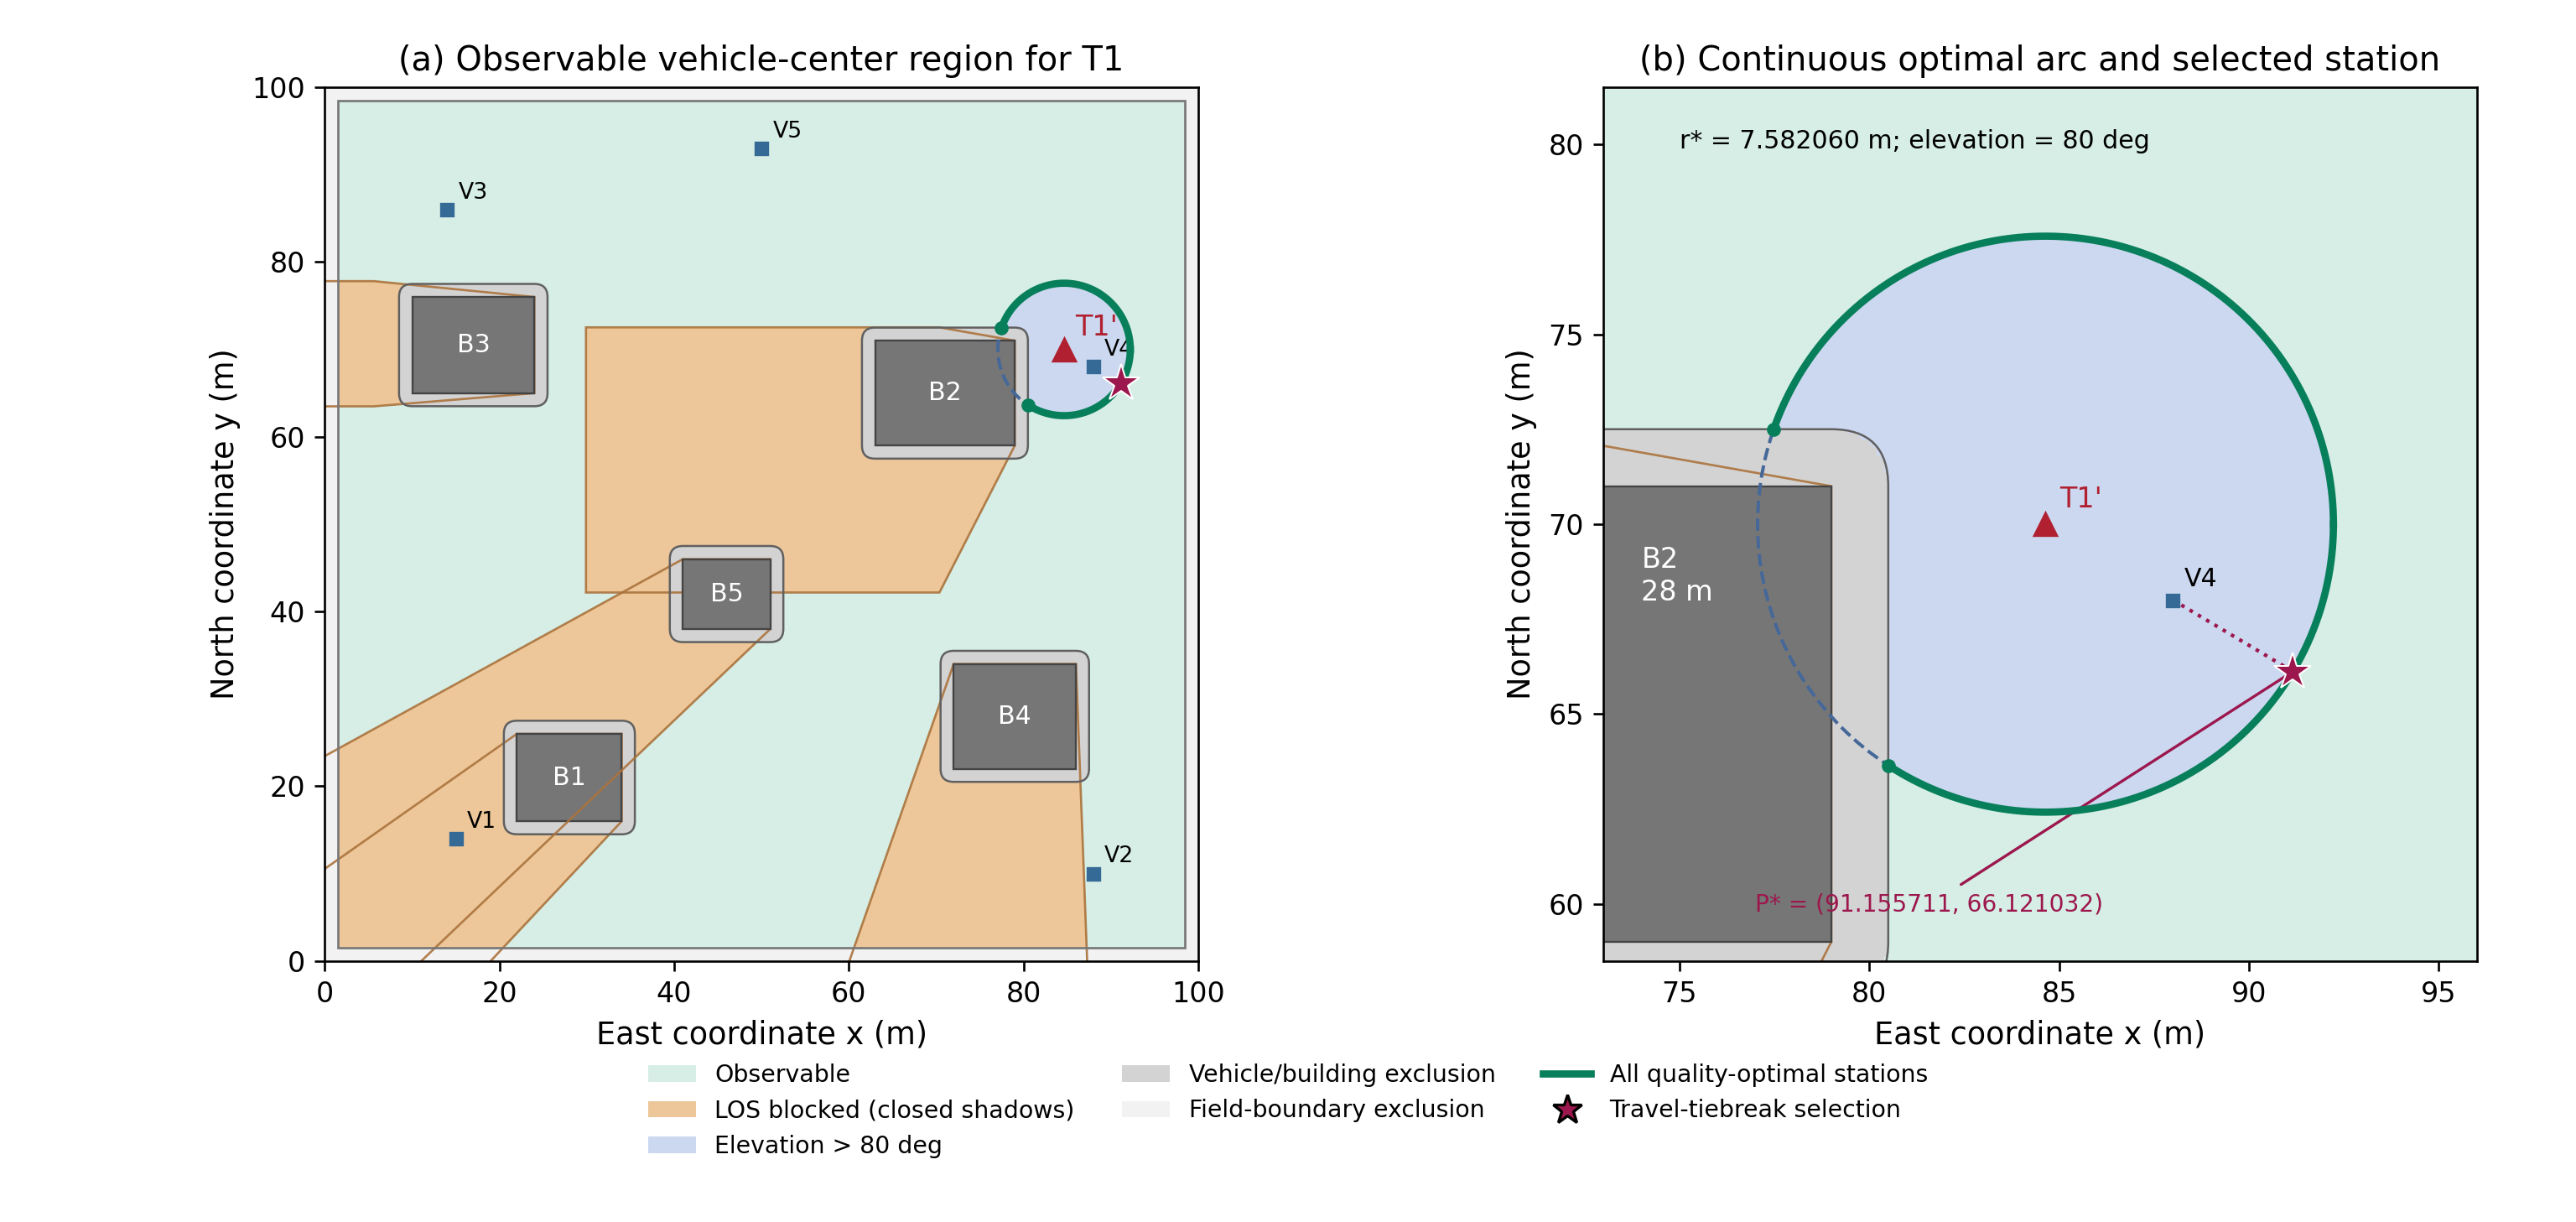
\includegraphics[width=\linewidth]{figures/Q1-Observable-Region.png}
    \caption{Observable vehicle centers for \(T_1\) and the continuous optimal arc. In (b), the dotted line shows the 3.673 m drive from \(V_4\) to the selected station (star). The green dots are the included endpoints of the optimal arc. Shading uses a 0.1 m grid.}
    \label{fig:q1-observable-mtdc}
\end{figure}

Maximizing \(Q(p)=1/r_1(p)\) over \(\mathcal A_1\) is equivalent to minimizing \(r_1(p)\). The point due east of \(T'_1\) at radius \(43\cot80^\circ\) lies in \(\mathcal A_1\), so the elevation bound is attained. The optimal values are
\begin{equation}
\label{eq:q1-optimal-values}
r^*=43\cot80^\circ\simeq 7.582060170\,\mathrm m,\qquad
Q^*\simeq 0.131890275\,\mathrm{m^{-1}},\qquad \beta^*=80^\circ.
\end{equation}
On the optimal circle, the field boundary and four of the five vehicle exclusion regions impose no further restriction. The offset edges \(y=72.5\) and \(x=80.5\) of \(B_2\) determine the endpoints. Intersecting the circle with the five shadows gives only the blocked segment from \(B_2\), approximately \([169.947439^\circ,221.927136^\circ]\), wholly within the excluded vehicle arc. Write \(p(\varphi)=T'_1+r^*(\cos\varphi,\sin\varphi)\), with angles measured counterclockwise from east. The feasible angles are
\begin{equation}
\label{eq:q1-feasible-arc}
[0^\circ,160.747873^\circ]\ \cup\ [236.896047^\circ,360^\circ),
\end{equation}
with endpoint angles rounded for display. These intervals join across \(0^\circ\) to form one arc that includes both vehicle tangency endpoints.

Among stations attaining \(Q^*\), the minimum travel distance criterion (MTDC) selects the vehicle and station with the shortest feasible drive. Any remaining tie is resolved by vehicle index, then by \(x\) and \(y\) in ascending order. From an initial center \(p_i^0\), the reverse triangle inequality gives \(\bigl|\|p_i^0-T'_1\|-r^*\bigr|\) as a lower bound on travel to any point on the circle. This bound is smallest for \(V_4\), which starts at \((88,68)\,\mathrm m\). Its radial projection lies on the feasible arc. Along the straight segment to that station, the disk stays inside the field and never extends west of \(x=86.5\,\mathrm m\), while every building footprint ends at \(x\le 86\,\mathrm m\). The drive therefore attains the lower bound of \(3.672741496\,\mathrm m\). The station is
\begin{equation}
\label{eq:q1-selected-station}
p^*=T'_1+r^*\frac{p_4^0-T'_1}{\|p_4^0-T'_1\|}
    \simeq(91.155710853,66.121032434)\,\mathrm m.
\end{equation}
\hyperref[app:q1-alternatives]{Appendix~B.1} gives the clearance-based tie-break and independent geometry checks.

% 正西—正北站对底表见 results/q2/正西正北等精度站对_20261122/。
\subsection{Two-Station Localization for \texorpdfstring{\(T_2\)}{T2}}
\label{sec:q21-model}

Two intersecting bearing lines estimate the horizontal coordinates of \(T_2\). Its alert supplies the height used in the visibility and elevation tests in Section~\ref{sec:q1-model}. For station \(p_i\), let \(r_i=\|T'_2-p_i\|\) be the horizontal range and \(\alpha_i\) the bearing to the target. A small target displacement \(\delta t\) changes that bearing by \(n_i^{\mathsf T}\delta t/r_i\), where \(n_i=(-\sin\alpha_i,\cos\alpha_i)^{\mathsf T}\). The Jacobian \(J\) stacks the two rows \(n_i^{\mathsf T}/r_i\)~\cite{ref:bearing-geometry}. The bearing errors are independent, zero-mean Gaussian variables with standard deviation \(\sigma_\theta=\pi/180\) radians.

For a noncollinear pair, first-order error propagation gives
\begin{equation}
\label{eq:q21-linearized-error}
\Sigma_{\rm lin}=\sigma_\theta^2(J^{\mathsf T}J)^{-1},\qquad
E_{\rm lin}=\sqrt{\operatorname{tr}\Sigma_{\rm lin}}
    =\frac{\sigma_\theta\sqrt{r_1^2+r_2^2}}{|\sin\gamma|},
\end{equation}
where \(\gamma\) is the angle between the two directed bearings. The trace measures the expected squared length of the linearized horizontal error, independent of the coordinate axes. Baseline length \(B=\|p_1-p_2\|\) enters through \(B^2=r_1^2+r_2^2-2r_1r_2\cos\gamma\). At fixed ranges, the error is smallest at \(B=\sqrt{r_1^2+r_2^2}\), where the bearings meet at \(90^\circ\). At a fixed angle, increasing either range increases the error.

Since \(H_2=35\,\mathrm m\), each feasible station has \(r_i\ge r_0=33\cot80^\circ\simeq5.818790363\,\mathrm m\). Thus
\begin{equation}
\label{eq:q21-error-lower-bound}
E_{\rm lin}\ge\sqrt{2}\,\sigma_\theta r_0\simeq0.143623358\,\mathrm m.
\end{equation}
Equality requires orthogonal bearings with both ranges equal to \(r_0\). A feasible pair places \(V_3\) due west of \(T'_2=(50-45\sqrt{3}/2,72.5)\) and \(V_5\) due north, at \(T'_2+(-r_0,0)\) and \(T'_2+(0,r_0)\), respectively. Below the roof height of \(B_3\), one sight segment passes west of the building and the other passes north. Both clear the remaining buildings. The straight routes in Table~\ref{tab:q21-west-north} each take less than the allowed 30 s. With simultaneous departures and the other three vehicles remaining at their origins, the minimum center separation throughout deployment is \(8.229012\,\mathrm m\). The pair attains the global minimum of \(E_{\rm lin}\) with an \(8.229012248\,\mathrm m\) baseline, a \(90^\circ\) intersection and two \(80^\circ\) elevations.

\begin{table}[!htbp]
    \centering
    \caption{West--north station pair for \(T_2\). Coordinates are rounded for display. Clearance is the shortest distance from the vehicle body to a building along the route.}
    \label{tab:q21-west-north}
    \setlength{\tabcolsep}{4pt}
    \begin{tabular}{@{}lccrrr@{}}
        \toprule
        Vehicle & Initial center (m) & Station (m) & \shortstack[r]{Drive\\length (m)}
            & \shortstack[r]{Drive\\time (s)} & \shortstack[r]{Building\\clearance (m)} \\
        \midrule
        \(V_3\) & \((14,86)\) & \((5.210066,72.500000)\) & 16.109405 & 5.369802 & 0.604320 \\
        \(V_5\) & \((50,93)\) & \((11.028857,78.318790)\) & 41.644783 & 13.881594 & 0.818790 \\
        \bottomrule
    \end{tabular}
\end{table}

As \(\gamma\) approaches \(0^\circ\) or \(180^\circ\), \(1/|\sin\gamma|\) amplifies bearing error. At either endpoint \(J\) loses rank and the target's position along the common line is undetermined. Screening by intersection angle or condition number flags this geometric failure. Away from the linear regime, nearly parallel noisy bearings can give long-tailed intersection errors, which can be assessed with error quantiles. A station on an included boundary of \(\mathcal A_2\) does not by itself cause rank loss: \(|\det J|=|\sin\gamma|/(r_1r_2)\). The west--north pair remains full rank at the \(80^\circ\) limit. A sight line that touches a building is infeasible. To avoid crossing a boundary when rounding, retain exact coordinates for the analysis and check rounded deployment coordinates after adding a margin toward the feasible interior. The clearance-binding pair in \hyperref[app:q21-alternatives]{Appendix~B.2} attains the same RMSE and shortens the longer drive from \(13.882\) to \(13.294\,\mathrm s\). Moving both stations of that pair radially outward before rounding gives a verified millimeter deployment with an RMSE of \(0.146102\,\mathrm m\).

% 毫米与全精度排程、就近基线：results/q2/毫米部署与初排_全程净空四十五厘米_20261121/。
% 连续下界：results/q2/等精度快速部署与并发排程_20261121/continuous_bound.json。
\subsection{Concurrent Assignment and Routing for Three Alerts}
\label{sec:q22-model}

Three alerts released at \(t=0\) create six observation slots for five vehicles. At least one vehicle must finish an observation, reset its gimbal and become ready for a second assignment. This dependency couples station selection and scheduling. The objective is to minimize the latest of the synchronized starts, \(t_{\rm last}=\max_m t_m^{\rm start}\).

At station \(p\), let \(\alpha_m(p)\) be the shortest signed pan angle from due east and \(\beta_m(p)\) the elevation, both in degrees. Pan and tilt run concurrently. Slewing from the travel attitude of due east and level, and resetting to it after an observation, each take
\begin{equation}
\label{eq:q22-slew-time}
\tau_m(p)=\frac{\max\{|\alpha_m(p)|,|\beta_m(p)|\}}{30^\circ/\mathrm s}.
\end{equation}
For \(V_i\) assigned to \(T_m\), write \(d_{im}\) for departure time, \(L_{im}\) for obstacle-avoiding route length and \(p_{im}\) for the station. The arrival time \(a_{im}\), readiness time \(u_{im}\) and joint start satisfy
\begin{equation}
\label{eq:q22-joint-start}
a_{im}=d_{im}+\frac{L_{im}}{3\,\mathrm{m/s}},\qquad
u_{im}=a_{im}+\tau_m(p_{im}),\qquad
t_m^{\rm start}=\max_{i\in\mathcal K_m} u_{im},
\end{equation}
where \(\mathcal K_m\) is the assigned vehicle pair. Vehicles may depart at \(t=0\) for their first assignments. For a reused vehicle, the next departure follows the previous joint start, 5 s of observation and its own reset. Each station lies in \(\mathcal A_m\), and each pair must have noncollinear bearings. Vehicle centers must stay at least 3 m apart during travel and parking.
% 条件性净空算例见 docs/B题第二至四问_撞墙风险与净空验收.md；0.40 m 并非实测误差。
To keep both schedules away from contact, we require \(0.45\,\mathrm m\) of nominal clearance from the vehicle body to buildings and the field boundary during travel and parking. This is an added planning margin, not a requirement in the problem. If combined map, vehicle-envelope and path-tracking errors were bounded by \(0.40\,\mathrm m\), at least \(0.05\,\mathrm m\) would remain; the error bound is illustrative, not measured.

A branch-and-bound search~\cite{ref:branch-and-bound} considers the six alert orders and their vehicle and station assignments. Candidate grids have spacings of 5, 2.5 and 1.25 m and include the vehicle origins and supplementary stations. A visibility graph~\cite{ref:visibility-graph} around conservatively inflated footprints provides route lengths. Lower bounds on readiness and transfers prune assignments that cannot improve the best schedule found so far. The alert order constrains shared vehicles. Vehicles on separate assignments can prepare in parallel.

The search identifies \(V_3:T_1\to T_3\) as the chain that determines the latest start. Sequential quadratic programming~\cite{ref:sqp} refines the two stations of \(V_3\) with its first partner, \(V_5\), fixed. The objective includes the first joint start, observation, reset, transfer and second slew. After refining the chain, the remaining three vehicles fill the other slots within its time limit. Shorter total driving distance determines the choice among the tested completions.

At least one vehicle must serve twice, giving 30 possible ordered pairs of successive alerts across the five vehicles. Bounding travel and pointing times on each chain gives a continuous-domain lower bound of \(10.352100\,\mathrm s\) (\hyperref[app:q22-bound]{Appendix~C.1}). The full-precision schedule reaches \(10.352118514\,\mathrm s\), within \(18.514\,\mu\mathrm s\) of that bound.

Before rounding the deployment to millimeters, the refinement adds \(0.10\,\mathrm m\) of station margin for parking, visibility and the radial elevation limit, with allowances for rounding. Independent replay at the rounded coordinates checks sight segments, gimbal phases, route clearance and continuous vehicle separation. The minimum optical margin is \(0.100852\,\mathrm m\). The minimum body clearances to buildings and the field boundary are \(5.780\,\mathrm m\) and \(5.500\,\mathrm m\), respectively, and the minimum vehicle-center separation is \(33.446\,\mathrm m\).

\begin{table}[!htbp]
    \centering
    \caption{Five-vehicle millimeter deployment used in Section~\ref{sec:q4-model}. Paired times are read from top to bottom, in seconds. Slewing starts at arrival and resetting starts at the end of joint observation. A dash indicates parking after the final reset.}
    \label{tab:q22-millimeter}
    \setlength{\tabcolsep}{3pt}
    \begin{tabular}{@{}lcrrrrr@{}}
        \toprule
        \shortstack[l]{Vehicle\\and alert} & Station (m) & \shortstack[r]{Departure\\arrival}
            & \shortstack[r]{Slew\\ends} & \shortstack[r]{Joint start\\and end}
            & \shortstack[r]{Reset\\ends} & \shortstack[r]{Next\\departure} \\
        \midrule
        \(V_1/T_2\) & \((15.000,14.000)\) & \shortstack[r]{0\\0} & 3.129448
            & \shortstack[r]{6.927598\\11.927598} & 15.057046 & --- \\
        \(V_2/T_3\) & \((88.000,10.000)\) & \shortstack[r]{0\\0} & 5.777589
            & \shortstack[r]{10.391510\\15.391510} & 21.169099 & --- \\
        \(V_3/T_1\) & \((15.033,87.088)\) & \shortstack[r]{0\\0.500093} & 1.532122
            & \shortstack[r]{1.532122\\6.532122} & 7.564152 & 7.564152 \\
        \(V_3/T_3\) & \((16.824,88.760)\) & \shortstack[r]{7.564152\\8.380871} & 10.391510
            & \shortstack[r]{10.391510\\15.391510} & 17.402149 & --- \\
        \(V_4/T_2\) & \((88.064,70.901)\) & \shortstack[r]{0\\0.967235} & 6.927598
            & \shortstack[r]{6.927598\\11.927598} & 17.887962 & --- \\
        \(V_5/T_1\) & \((50.000,93.000)\) & \shortstack[r]{0\\0} & 1.532033
            & \shortstack[r]{1.532122\\6.532122} & 8.064155 & --- \\
        \bottomrule
    \end{tabular}
\end{table}

Table~\ref{tab:q22-millimeter} lists the events of the millimeter-coordinate schedule. Section~\ref{sec:test-scheduling} compares the two schedules on a common time axis. A vehicle that finishes slewing before its partner waits until the joint start. Only \(V_3\) and \(V_4\) drive, on three straight legs totaling \(6.852140\,\mathrm m\). The first legs start at \((14,86)\) and \((88,68)\,\mathrm m\), respectively, and the second leg of \(V_3\) links its two stations in the table. The last alert starts at \(10.391510\,\mathrm s\), \(39.391\,\mathrm{ms}\) after the full-precision schedule.

The nearest-assignment baseline selects for each alert the feasible pair with the smallest sum of added route lengths from the vehicles' origins or previous stations. Earlier joint readiness breaks distance ties, followed by a fixed ordering of vehicles and stations. The search enforces the common timing and 0.45 m vehicle-body clearance requirements. Independent replay also confirms that the six resulting zero-drive plans meet the 0.10 m station margins. The best processing order is \(T_1,T_2,T_3\), with respective joint starts of \(1.532033\), \(10.968984\) and \(5.777589\,\mathrm s\) at the vehicles' initial positions. Its pairs are \(V_3,V_5\) for \(T_1\), \(V_1,V_3\) for \(T_2\), and \(V_2,V_4\) for \(T_3\).

\hyperref[app:q22-alternatives]{Appendix~B.3} gives the fixed-partner and multistart schedules.

At its second observation, \(V_3\) has driven \(3.950\,\mathrm m\) cumulatively and its station lies \(86.862\,\mathrm m\) horizontally from \(T_3\). In Section~\ref{sec:q3-model}, cumulative travel controls how localization error grows, and station-to-target range controls how that error translates into an angle. Section~\ref{sec:q4-model} starts from the same schedule and reconstructs the vehicle states at the disturbance time.

% 可靠性阈值与误差贡献：results/q3/测向可靠性与80米定位约束_五方法对照_20261120/。
\subsection{Bearing Reliability and the Travel Limit}
\label{sec:q3-model}

Problem~3 fixes the horizontal station-to-target range at \(D=40\,\mathrm m\). Take the true vehicle position as the origin and align the positive \(x\)-axis with the true sight line. After cumulative travel \(s\), the two components \((\delta_x,\delta_y)\) of the position-estimation error are independent zero-mean Gaussian variables with per-axis standard deviation \(\sigma(s)=0.30+0.02s\) in meters. The estimated sight vector is \((D-\delta_x,-\delta_y)\). With \(W\) wrapping angles to \([-\pi,\pi)\), the deviations are
\begin{equation}
\label{eq:q3-bearing-deviations}
\alpha=\operatorname{atan2}(-\delta_y,D-\delta_x),\qquad
\Delta\psi_{\rm cmd}=W(\alpha),\qquad
\Delta\psi_{\rm act}=W(\alpha+G).
\end{equation}
The problem defines \(\Delta\psi\) as the commanded-bearing deviation. For actual pointing, \(G\) adds the gimbal zero-offset and control errors. They are independent zero-mean Gaussian variables and are independent of the position error. Their standard deviations of \(0.8^\circ\) and \(0.6^\circ\) combine to \(g=1^\circ=\pi/180\) radians. These deviations describe the pointing at a single observation. Section~\ref{sec:q21-model} models the separate bearing measurement used for intersection.

For \(\sigma>0\), integration of the Gaussian sight-vector density over the radius gives the projected-normal angular density~\cite{ref:projected-normal}. With \(\kappa=D/\sigma\) and standard normal distribution function \(\Phi\),
\begin{equation}
\label{eq:q3-projected-normal-density}
f_\kappa(u)=\frac{e^{-\kappa^2/2}}{2\pi}
    +\frac{\kappa\cos u}{\sqrt{2\pi}}e^{-\kappa^2\sin^2 u/2}\Phi(\kappa\cos u),
    \qquad -\pi\le u<\pi.
\end{equation}
Set \(h=5\pi/180\). At a commanded deviation of \(u\), actual pointing meets the tolerance when \(u+G\) falls within \(h\) of an integer multiple of \(2\pi\). The conditional success probability is
\begin{equation}
\label{eq:q3-conditional-coverage}
K_g(u)=\sum_{\ell\in\mathbb Z}\left[
\Phi\!\left(\frac{h-u+2\ell\pi}{g}\right)
-\Phi\!\left(\frac{-h-u+2\ell\pi}{g}\right)\right].
\end{equation}
The two coverage probabilities reduce to one-dimensional integrals,
\begin{equation}
\label{eq:q3-coverage-integrals}
R_{\rm cmd}(\sigma)=\int_{-h}^h f_\kappa(u)\,\mathrm du,\qquad
R_{\rm act}(\sigma)=\int_{-\pi}^{\pi} f_\kappa(u)K_g(u)\,\mathrm du.
\end{equation}
Using the same standard normal samples \(Z_x,Z_y\) at different \(\sigma\), the absolute commanded deviation is distributed as \(\operatorname{atan2}(|Z_y|,D/\sigma+Z_x)\). It increases almost surely with \(\sigma\), with positive probability of crossing the fixed tolerance between any two distinct positive values of \(\sigma\). Actual-pointing coverage also decreases strictly because \(K_g(u)\) decreases with angular distance from zero. Both probabilities start above 0.95 at \(\sigma=0\) and tend to \(h/\pi\), so each has a unique 95\% threshold.

Adaptive quadrature~\cite{ref:adaptive-quadrature} uses symmetry and subdivisions near the narrow density peak and tolerance edges. At the nominal gimbal standard deviation, retaining the central window in \(K_g\) omits at most \(2\Phi(-175)\) of conditional probability. Brent's method~\cite{ref:brent} gives the root \(\sigma_*\) of \(R(\sigma_*)=0.95\), and \(s_{\max}=(\sigma_*-0.30)/0.02\). Evaluations \(0.01\,\mathrm m\) below and above each travel limit give probabilities on the corresponding sides of the threshold. \hyperref[app:q3-alternatives]{Appendix~B.4} gives the independent checks.

\begin{table}[!htbp]
    \centering
    \caption{Travel limits and 80 m coverage probabilities at a horizontal target range of 40 m.}
    \label{tab:q3-limits}
    \begin{tabular}{@{}lrrr@{}}
        \toprule
        Bearing definition & Critical \(\sigma_*\) (m) & \shortstack[r]{Maximum\\travel (m)} & \shortstack[r]{Probability\\at 80 m} \\
        \midrule
        Commanded bearing & 1.778721312 & 73.936066 & 93.347323\% \\
        Actual pointing   & 1.636745169 & 66.837258 & 91.506823\% \\
        \bottomrule
    \end{tabular}
\end{table}

Fig.~\ref{fig:q3-travel-reliability} shows where each curve crosses the \(95\%\) requirement. At 80 m both curves lie below it, with the lower coverage for actual pointing because its error includes the two gimbal terms.

% q3 以论文采用的 D=40 m 工况绘图，沿用归档 reliability.pdf 的曲线、阈值和 80 m 标记。
\begin{figure}[!htbp]
    \centering
    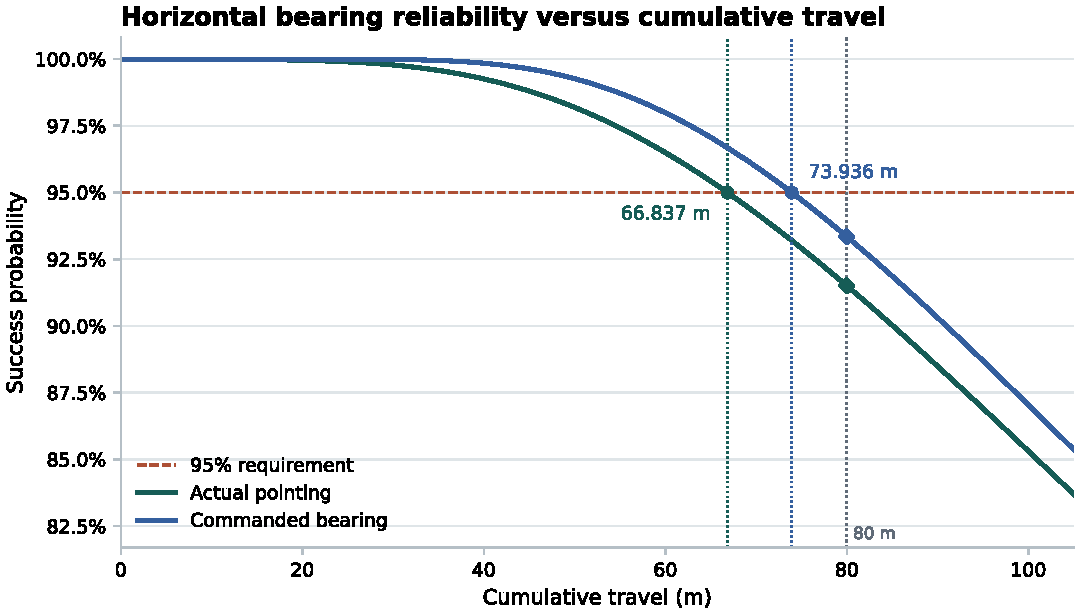
\includegraphics[width=0.78\linewidth]{figures/Q3-Bearing-Reliability.pdf}
    \caption{Probability of staying within \(5^\circ\) of the true bearing at a horizontal target range of 40 m. Circles mark the 95\% travel limits and diamonds mark coverage at 80 m.}
    \label{fig:q3-travel-reliability}
\end{figure}

At 80 m the nominal per-axis standard deviation reaches \(1.90\,\mathrm m\). For \(\sigma(s)=a+bs\) with \(a,b\ge0\), the 95\% requirement at each given cumulative distance through 80 m is equivalent to
\begin{equation}
\label{eq:q3-parameter-domain}
a+(80\,\mathrm m)b\le\sigma_*,\qquad
\sigma_*\simeq\begin{cases}
1.778721312\,\mathrm m & \text{for commanded bearing},\\
1.636745169\,\mathrm m & \text{for actual pointing}.
\end{cases}
\end{equation}
With the initial localization standard deviation fixed at \(a=0.30\,\mathrm m\), the drift coefficient \(b\) must be at most \(0.0184840\,\mathrm{m/m}\) for commanded bearing and \(0.0167093\,\mathrm{m/m}\) for actual pointing. The nominal value \(b=0.020\,\mathrm{m/m}\) exceeds both limits. Fig.~\ref{fig:q3-parameters-80m} in \hyperref[app:q3-alternatives]{Appendix~B.4} shows the two feasible regions.

Transverse position error supplies the leading localization term because \(\alpha\simeq-\delta_y/D\). In squared degrees, the first-order variances from localization, zero offset and control are \((180\sigma/(\pi D))^2\), \(0.8^2\) and \(0.6^2\). Their shares of the actual-pointing variance are \(15.59\%\), \(54.02\%\) and \(30.39\%\) at departure, changing to \(88.10\%\), \(7.61\%\) and \(4.28\%\) after 80 m. Recomputing the nonlinear probability at 80 m after removing each source individually raises actual-pointing coverage by \(8.493\), \(1.181\) and \(0.665\) percentage points, respectively. Zero-offset calibration addresses the largest contribution at departure. Reducing localization drift or re-localizing before observation has the largest effect at 80 m. The commanded bearing depends only on the position estimate, so the two gimbal terms contribute zero to its variance.

With the same angular noise at other ranges, coverage depends on \(D\) and \(\sigma\) through \(D/\sigma\). The critical standard deviation therefore scales as \(\sigma_*(D)=\sigma_*(40\,\mathrm m)D/(40\,\mathrm m)\). This relation gives a pointing check for an assigned vehicle from its station-to-target range and cumulative travel.

% 情景比分与独立回放：results/q4/毫米初排与联合断联限制_全程净空四十五厘米_20261121/。
% 同初排逐场配对：results/q4/同毫米初排分区与全场配对_20261122/paired_cases.csv。
\subsection{Field-Wide Rescheduling under Disturbances}
\label{sec:q4-model}

\subsubsection{Dispatch State and Scoring}

At \(t=5\,\mathrm s\) in Table~\ref{tab:q22-millimeter}, \(V_3\) and \(V_5\) are observing \(T_1\), \(V_1\) is waiting for its partner at the \(T_2\) station, and \(V_2\) and \(V_4\) are still slewing. Field-Wide Rescheduling (FW) and strict retention (SR) start from the same millimeter-coordinate schedule, without advance information about the disturbance. A failed vehicle immediately withdraws from service and leaves routes unobstructed. A new alert adds a two-vehicle task.

The rescheduling policy is event-driven~\cite{ref:rescheduling}. With communication available, revised commands take effect at 5 s. During an outage, they take effect at \(t_{\rm rec}\). The Problem B author clarified that \(t_{\rm rec}\in(5,30]\,\mathrm s\) is the recovery time measured from \(t=0\), so the outage lasts \(t_{\rm rec}-5\,\mathrm s\)~\cite{ref:problem-b-outage}. The main outage rule uses the queue authorization and readiness confirmation assumptions in Section~\ref{sec:assumptions}. The joint restriction defers departures that have yet to occur at 5 s and new joint starts until recovery; Section~\ref{sec:q4-outage-sensitivity} also examines each restriction separately. If recovery coincides with a departure or a joint start, the dispatcher reads the state first.

At dispatch, replay reconstructs each vehicle's position, gimbal attitude, remaining route and task phase. Any observation started strictly before dispatch is locked, including starts confirmed by the original partners during an outage. If a failure interrupts a locked observation, its start still counts and the healthy partner remains committed through the original observation slot and its own reset.

Let \(f_i\) be the earliest release time of a healthy vehicle and \(b_{im}\) its preparation time for a new assignment after release. A vehicle that leaves its position resets to due east and level if necessary, drives, then slews. A vehicle that stays can slew from its current attitude. When a moving vehicle retains its destination, it follows the remainder of the original route. The joint start and the next release time for a candidate pair are
\begin{equation}
\label{eq:q4-dispatch-times}
t_m^{\rm start}=\max_{i\in\mathcal K_m}(f_i+b_{im}),\qquad
f_i^{\rm next}=t_m^{\rm start}+5\,\mathrm s+\tau_m(p_{im}),\quad i\in\mathcal K_m.
\end{equation}
Reported times assume zero computation and command latency. Given \(N\) alerts, including \(T_4\) when present, \(k\) counts synchronized starts strictly before 60 s. Plans rank by higher \(\eta=k/N\), then by smaller \(t_{\rm last}\). If all alerts start, \(t_{\rm last}=\max_m t_m^{\rm start}\). Otherwise the score assigns \(t_{\rm last}=60\,\mathrm s\). A separate metric counts observations with 5 uninterrupted seconds of overlap between the two vehicle recordings within the window. SR follows the original assignments, stations, routes and order under the applicable communication rule. A failed partner's slot stays vacant, and a new alert stays unassigned.

\subsubsection{Field-Wide Search and Replay}

FW selects vehicle pairs, stations and service order for pending alerts. Candidate stations include original stations, initial and current vehicle positions, and sites sampled across the field. New station pairs must satisfy observability, at least 3 m of separation and \(5^\circ<\gamma<175^\circ\). Transfers use the visibility graph from Section~\ref{sec:q22-model}, with \(0.45\,\mathrm m\) nominal body clearance along routes and at stations.

Each beam-search layer~\cite{ref:beam-search} assigns one pending alert to a vehicle pair and updates both vehicles' stations and release times. Finalists rank by scenario score, with ties broken by the smaller sum of start times. In that order, continuous replay checks station geometry, gimbal timing, route clearance and vehicle separation until a feasible schedule is found. \hyperref[app:q4-search-settings]{Appendix~D.5} gives the sampling and search settings.

\subsubsection{Disturbance Scenarios and Scores}

The scenario set samples 24 equally spaced azimuths for \(T_4\), three ranges of 30, 40 and 50 m, and the specified height of 50 m. Conditional on a failure, the five vehicles are equally likely to fail, and each identity is tested. Recovery at 10, 20 and 30 s gives outage lengths of 5, 15 and 25 s, with recovery on both sides of the undisturbed last start at \(10.391510\,\mathrm s\). The disturbance options include the absence of each disturbance. Their combinations, excluding the undisturbed case, give \(73\times6\times4-1=1{,}751\) scenarios. Reported means weight each scenario equally.

\begin{table}[!htbp]
    \centering
    \caption{FW and SR results across the 1,751 main-rule scenarios. The mean score includes a 60 s penalty value wherever any alert fails to start.}
    \label{tab:q4-main-scores}
    \begin{tabular}{@{}lrr@{}}
        \toprule
        Metric & FW & SR \\
        \midrule
        Scenarios with every alert started & 1,751 & 7 \\
        Scenarios with all five-second recordings complete & 1,167 & 3 \\
        Mean latest-start score (s) & 24.746 & 59.802 \\
        \bottomrule
    \end{tabular}
\end{table}

Table~\ref{tab:q4-main-scores} compares the policies on the same scenarios. FW starts more alerts in 1,744 scenarios and ties SR in the other seven. Its maximum latest start is \(40.330\,\mathrm s\). In the 584 FW scenarios without complete recordings, a failure of \(V_3\) or \(V_5\) at 5 s cuts the already-started \(T_1\) recording to \(3.468\,\mathrm s\). Table~\ref{tab:q4-representative-scores} in Appendix~A gives the representative scores.

\subsubsection{Dispatch Decisions and Outage Effects}
\label{sec:q4-dispatch-effects}

In Case~10, \(T_1\) and \(T_2\) are locked at recovery at 10 s, and \(V_3\) is still slewing at its original \(T_3\) station. Under SR it waits at that station after the slew because \(V_2\) has failed. FW keeps \(V_3\)'s station and assigns \(V_5\) to point at \(T_3\) from its current position, \((50,93)\,\mathrm m\). The replacement pair starts at \(12.765521\,\mathrm s\).

More starts can come at the cost of delaying an original alert. In Case~08, SR starts \(T_3\) at \(10.391510\,\mathrm s\) and leaves \(T_2,T_4\) without a joint start. FW uses \(V_3,V_5\) for \(T_4\) at \(12.666382\,\mathrm s\) and reuses both for \(T_3\). Observation, reset, transfer and the next slew put the \(T_3\) start at \(23.185928\,\mathrm s\). The score rises from two to four starts while \(T_3\) starts \(12.794\,\mathrm s\) later. Cases~06 and~07 give identical start scores under FW and SR. In Case~06, the failed \(V_5\) has no later trip. In Case~07, the preauthorized queue has already started every alert by the time communication returns.

In Case~12, \(T_3\) starts at \(10.391510\,\mathrm s\) and \(V_2\) finishes its observation and reset before communication returns at 30 s. The dispatcher therefore locks \(T_3\). In Case~12R, \(T_3\) is pending at recovery and \(V_2\) is waiting in its \(T_3\) pointing attitude. FW assigns \(T_3\) to \(V_3,V_5\) and sends \(V_2\) to \(T_2\). The same \(T_2\) route for \(V_2\) now requires a \(5.777589\,\mathrm s\) cancellation reset before departure. Since \(V_2\) determines the \(T_2\) start in both schedules, the latest start moves from \(40.330420\) to \(46.108009\,\mathrm s\). Across the same 1,314 outage scenarios, imposing both restrictions raises the FW mean from \(26.436\) to \(32.301\,\mathrm s\). Under each rule, every alert starts in all 1,314 scenarios and every alert records for five uninterrupted seconds in 876.

By the start of \(T_4\) in Case~12R, \(V_3\) has accumulated \(10.167\,\mathrm m\) of travel and stands \(8.464\,\mathrm m\) horizontally from the target. With these values, the model in Section~\ref{sec:q3-model} predicts \(84.04\%\) actual-pointing coverage for that individual vehicle. The scenario scores four synchronized starts under the nominal timing and geometry used for scheduling.

\hyperref[app:q4]{Appendix~A} gives the dispatch decisions, stations and complete vehicle timelines for representative cases. \hyperref[app:q4-alternatives]{Appendix~B.5} compares the additional policies. Supplement~S4 in the supporting materials covers all 1,751 main scenarios and 1,314 joint-restriction replays. It provides the scores in \path{panel/scenario_scores.csv}, the decisions in \path{panel/decisions.jsonl.gz}, and the five-vehicle timelines in \path{panel/vehicle_timelines.csv.gz}.

\section{Test the Models}
\label{sec:model-tests}

% 据队员确认的提纲和讨论稿同步。GPT-6.2 Sol 辅助整理已有证据、英文措辞与排版。
\subsection{Observable Region and Station Selection}

% 遮挡对照及直达路线见 results/q1/最短行驶站与可观测区域_20261122/result.json。
% 面积上下界见 results/q1/可观测区域与最优站位_连续圆弧_20261120/area_check_continuous.json。
For \(T_1\), we tested the projected shadows in Fig.~\ref{fig:q1-observable-mtdc} by intersecting each three-dimensional sight segment with each building. The two methods agreed for all five buildings at all 250,000 sampled vehicle centers. A separate check of 36,000 points on the minimum-range circle reproduced the predicted arc membership. The radial projection of \(V_4\)'s initial position lay on the feasible arc, and the straight drive to it attained the smallest travel lower bound, \(3.673\,\mathrm m\).\footnote{GPT-6.2 Sol and GPT-6.2 Astra (OpenAI) assisted with organizing the archived checks, editing the English and presenting the figures in this section.}

To check how the shading in Fig.~\ref{fig:q1-observable-mtdc} represents area, we counted feasible cell centers on three grids. At spacings of 0.20, 0.10 and 0.05 m the estimates were \(5{,}649.440\), \(5{,}610.400\) and \(5{,}608.528\,\mathrm{m^2}\), respectively. Bounding the feasible length in each vertical strip gave a continuous-area interval of \([5{,}608.767083,\,5{,}608.774146]\,\mathrm{m^2}\) (\hyperref[app:q1-alternatives]{Appendix~B.1}). The grid used for the figure thus overestimates the area by about \(1.63\,\mathrm{m^2}\).

\subsection{Two-Station Localization}

% 采用正文的全精度正西—正北构型，见 results/q2/正西正北等精度站对_20261122/q21_result.json。
% 仿真以相同半径、交会角和测角噪声复算几何，不含行驶过程。见 results/q2/双站定位与并发调度_连续站位_20261120/q21_sensitivity.csv。
Both sight lines from the west and north stations to \(T_2\) were clear, and the drives took \(5.370\) and \(13.882\,\mathrm s\), within the \(30\,\mathrm s\) limit (Table~\ref{tab:q21-west-north}). To test the first-order error estimate, we fixed both ranges at \(5.819\,\mathrm m\) (rounded) and intersected the rays after adding independent Gaussian errors of standard deviation \(1^\circ\) to the two bearings. At the nominal \(90^\circ\) angle all 100,000 trials yielded a forward intersection. The sample horizontal RMSE was \(0.144079\,\mathrm m\), about \(0.32\%\) above the first-order prediction of \(0.143623\,\mathrm m\).

Repeating the geometric test at the same ranges with a \(1^\circ\) or \(179^\circ\) intersection angle put the intersection behind at least one station in \(23.855\%\) and \(42.634\%\) of trials, respectively. An error calculated only for the remaining intersections would omit these failures.

\subsection{Concurrent Scheduling}
\label{sec:test-scheduling}

% 毫米初排回放见 results/q2/毫米部署与初排_全程净空四十五厘米_20261121/independent_validation.json。
% 18.514 微秒的间隙对应全精度排程，见 results/q2/等精度快速部署与并发排程_20261121/continuous_bound.json。
Independent replay at the millimeter coordinates reconstructed each joint observation from the two vehicles' arrival and slew times. In the upper panel of Fig.~\ref{fig:q22-timeline-comparison}, \(V_2\) finished pointing at \(T_3\) at \(5.777589\,\mathrm s\) and waited for \(V_3\) until \(10.391510\,\mathrm s\). Both then observed through \(15.391510\,\mathrm s\) before resetting. Over the full trajectories the minimum vehicle-center separation was \(33.446\,\mathrm m\).

% 图来自 results/q2/毫米初排与就近基线_五车时序蓝灰配色_20261123/q22_timeline.pdf，与 4.3 的毫米部署表共用开测口径。
\begin{figure}[!htbp]
    \centering
    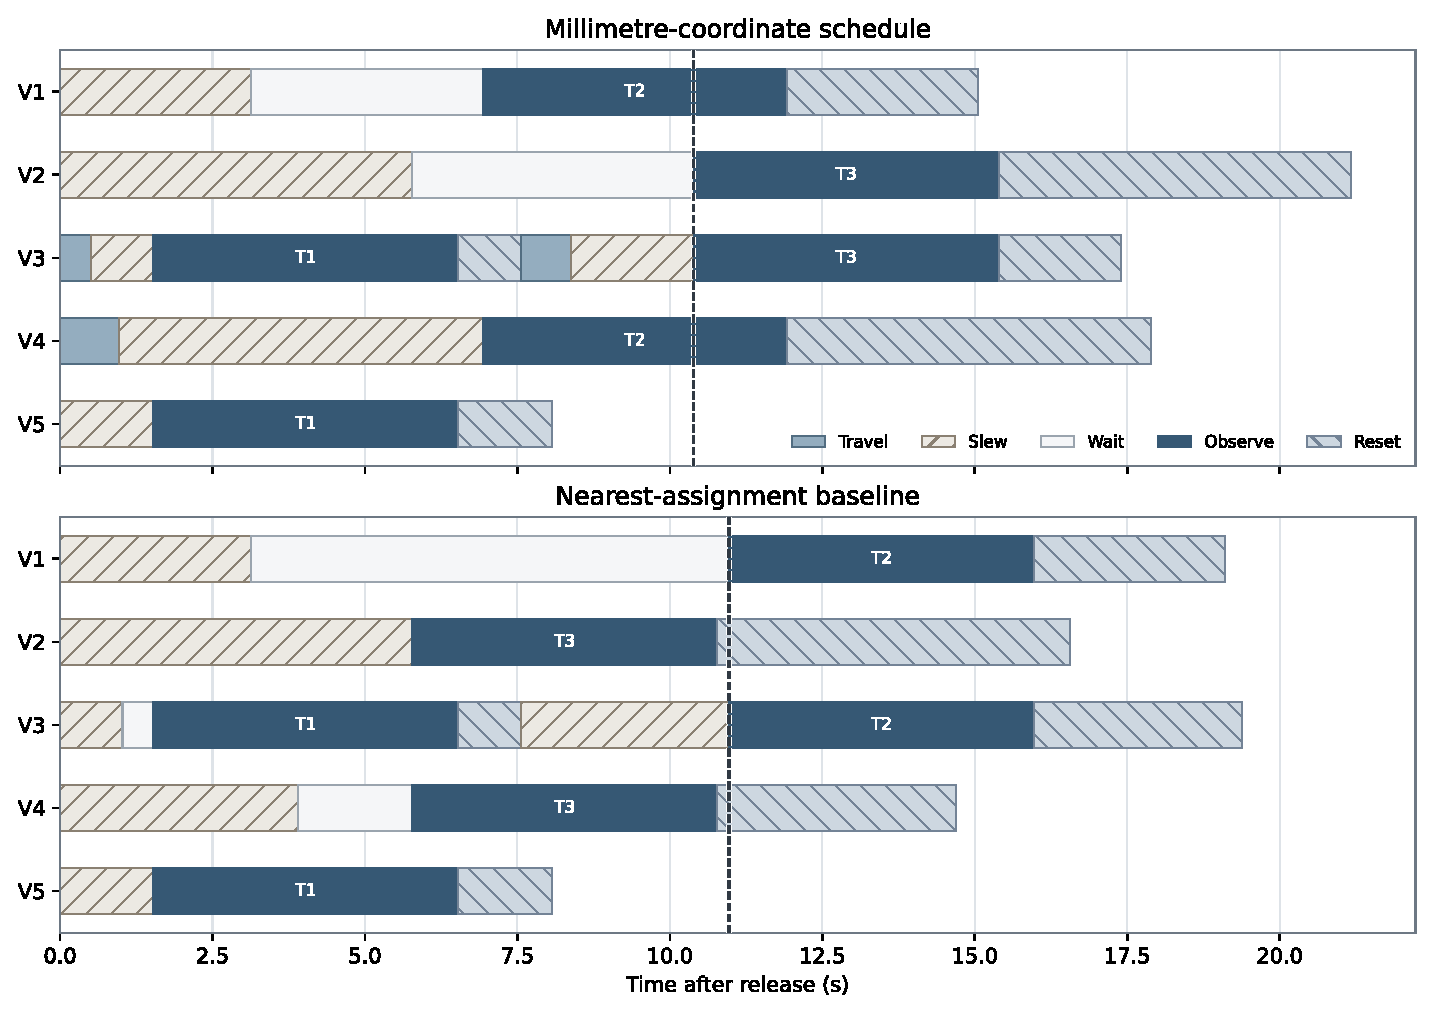
\includegraphics[width=0.87\linewidth]{figures/Q2-Five-Vehicle-Timelines.pdf}
    \caption{Five-vehicle timelines for the millimeter-coordinate schedule (top) and the nearest-assignment baseline (bottom). Dashed lines mark the latest joint starts at \(10.392\,\mathrm s\) for \(T_3\) and \(10.969\,\mathrm s\) for \(T_2\), respectively.}
    \label{fig:q22-timeline-comparison}
\end{figure}

In the baseline, \(V_3\) waits for \(V_5\) at \(T_1\) and needs another \(3.414\,\mathrm s\) after reset to point at \(T_2\). In the millimeter schedule, \(V_3\) uses part of that initial wait to drive for \(0.500\,\mathrm s\) before its first slew. Vehicles \(V_1,V_4\) take \(T_2\) in parallel, freeing \(V_3\) to take \(T_3\). Its transfer and second slew take \(2.827\,\mathrm s\) after reset. The last start moves from \(10.968984\) to \(10.391510\,\mathrm s\), a gain of \(0.577475\,\mathrm s\) (\(5.26\%\)). For the separate full-precision schedule, the latest start was \(18.514\,\mu\mathrm s\) above the continuous-domain lower bound (\hyperref[app:q22-bound]{Appendix~C.1}).

\subsection{Bearing Reliability}

% 半平面独立复算和临界值两侧检查见 results/q3/测向可靠性与80米定位约束_五方法对照_20261120/。
At a horizontal target range of \(40\,\mathrm m\), we checked the two crossings in Fig.~\ref{fig:q3-travel-reliability} by computing the acceptance probability from Gaussian half-planes. This calculation reproduced the travel limits of \(73.936066\,\mathrm m\) for commanded bearing and \(66.837258\,\mathrm m\) for actual pointing. For actual pointing, moving \(0.01\,\mathrm m\) below and above its limit gave probabilities of \(95.00237\%\) and \(94.99763\%\), respectively. The commanded-bearing check crossed the threshold in the same direction (\hyperref[app:q3-alternatives]{Appendix~B.4}).

Monte Carlo simulation used five million draws per test point. For both bearing definitions, the simultaneous confidence interval for coverage contained \(95\%\) at the calculated travel limit. It lay wholly above \(95\%\) at \(0.50\,\mathrm m\) below the limit and wholly below \(95\%\) at \(0.50\,\mathrm m\) above it (Fig.~\ref{fig:q3-test-mc} in \hyperref[app:q3-alternatives]{Appendix~B.4}).

\subsection{Rescheduling under Disturbances}

% 四种通信规则的完整验收见 results/q4/毫米初排与联合断联限制_全程净空四十五厘米_20261121/full_run_validation.json。
The rescheduling audit reconstructed \((\eta,t_{\mathrm{last}})\) from the vehicle timelines for 28,465 plans across 5,693 combinations of disturbance scenario and communication rule. Counting synchronized starts strictly before \(60\,\mathrm s\) reproduced the archived scores. Observations already underway retained their vehicle and station assignments, and revised commands took effect at or after communication recovery in the outage cases. The smallest vehicle-center separation over the continuous trajectories was \(3.241693\,\mathrm m\), against the required \(3\,\mathrm m\).

We also intersected the two vehicles' recording intervals to check how much data each scored start delivered. For example, \(T_1\) started at \(1.532122\,\mathrm s\). When either member of its pair failed at \(5\,\mathrm s\), the start still counted, but the uninterrupted joint recording lasted only \(3.467878\,\mathrm s\). This accounts for the difference in Table~\ref{tab:q4-main-scores} between the 1,751 main-rule scenarios in which field-wide rescheduling started every alert and the 1,167 in which every recording lasted the full five seconds.

\section{Sensitivity Analysis}
\label{sec:sensitivity}

% 经队员确认同步。OpenCode（Magpie, group/gpt-6.2-sol）于 2026-11-23 辅助数字复核、英文修订、热图和排版，供 AI 使用报告记录。
The sensitivity tests use the solutions in Section~\ref{sec:models} as baselines, with alternative solutions in \hyperref[app:alternatives]{Appendix~B}.

\subsection{Observable Area and Minimum-Travel Station Selection}
\label{sec:q1-sensitivity}

% 扰动输入及连续面积见 results/q1/仰角目标位置与净空敏感性_20261122/sensitivity.csv；原站及径向投影证书见 results/q1/最短行驶站与可观测区域_20261122/result.json。
% 固定站采用 MTDC 标称 V4 站，不使用敏感度 CSV 中的 MMCC 固定站列。逐行在最小半径圆上验收最近车辆的径向投影和直达路线。
Sixteen one-factor tests perturbed the upper elevation limit, the coordinates of \(T_1\), the roof height of \(B_2\), and the required parking clearance. The elevation limit varied by \(\pm0.5^\circ\) or \(\pm1^\circ\). The target coordinates varied by \(\pm0.5\,\mathrm m\) along either horizontal axis or by \(\pm1\) or \(\pm2\,\mathrm m\) vertically. The remaining tests varied the roof height by \(\pm1\,\mathrm m\) or imposed an additional clearance of \(0.10\) or \(0.45\,\mathrm m\). In each setting, the criterion in Section~\ref{sec:q1-model} selected the shortest feasible drive among stations that maximize \(Q=1/r\). A straight route from \(V_4\)'s initial position attained the travel-distance lower bound in all 16 tests.

Reducing the elevation limit from \(80^\circ\) to \(79^\circ\) increased the optimal horizontal range from \(7.582\) to \(8.358\,\mathrm m\) and the minimum driving distance from \(3.673\) to \(4.449\,\mathrm m\). The maximum observation quality and observable area decreased by \(9.29\%\) and \(0.54\%\), respectively. A \(1\,\mathrm m\) increase in the height of \(T_1\) expanded the observable area by \(1.29\%\). The greater minimum range in that setting reduced the maximum observation quality by \(2.27\%\). Raising the roof of \(B_2\) by \(1\,\mathrm m\) reduced the observable area by \(2.70\%\), with the nominal station still attaining both optimization objectives.

At the nominal station, the required elevation exceeded the applicable limit in six tests. These comprised the two reductions in the elevation limit, the two increases in target height, and the \(0.5\,\mathrm m\) shifts of \(T_1\) to the east and to the south. The nominal station satisfied the clearance and line-of-sight constraints in all 16 tests.

\subsection{Sensitivity of Two-Station Localization}

% 名义几何见 results/q2/正西正北等精度站对_20261122/；79° 复算将两站半径替换为 33 cot(79°)，按原方位独立验收。
For the west--north station pair in Section~\ref{sec:q21-model}, the first-order horizontal localization RMSE is proportional to the common standard deviation \(\sigma_\theta\) of the independent bearing errors. At the fixed stations, increasing \(\sigma_\theta\) from \(0.50^\circ\) to \(1.50^\circ\) increased the RMSE from \(0.071812\) to \(0.215435\,\mathrm m\). The prescribed standard deviation of \(1^\circ\) gives \(0.143623\,\mathrm m\).

Both nominal stations require an elevation of \(80^\circ\). At a \(79^\circ\) limit, radially displacing them along their original west and north directions increases the horizontal ranges to \(6.415\,\mathrm m\) and preserves the \(90^\circ\) intersection angle. The reselected pair attains the new first-order RMSE lower bound of \(0.158328\,\mathrm m\) at \(\sigma_\theta=1^\circ\), an increase of \(10.24\%\). The new stations satisfied the visibility constraints, and the simultaneous straight routes passed the clearance and vehicle-separation checks. The driving times for \(V_3\) and \(V_5\) were \(5.481\) and \(13.813\,\mathrm s\), respectively, within the individual \(30\,\mathrm s\) limit.

\subsection{Timing and Visibility of the Concurrent Schedule}

% 时序及高度扰动见 results/q2/毫米部署与初排敏感性_20261122/q22_sensitivity.csv。
Timing sensitivity was evaluated for the millimeter-coordinate schedule and the nearest-assignment baseline in Section~\ref{sec:q22-model}. Each replay used the assignments, stations, routes, and service order of the corresponding plan. Vehicle speed, gimbal angular speed, and observation duration each took five values between \(80\%\) and \(120\%\) of their nominal values, in increments of ten percentage points. Both plans were feasible in all 125 combinations. With the other inputs at their nominal values, a \(20\%\) increase in vehicle speed advanced the latest start of the millimeter-coordinate schedule by \(0.136\,\mathrm s\). A \(20\%\) increase in gimbal angular speed advanced it by \(0.679\,\mathrm s\).

Throughout the tested grid, each schedule's latest start depended on one preceding observation. An additional second of observation therefore delayed both latest starts by one second. The millimeter-coordinate schedule had the smaller \(t_{\mathrm{last}}\) at 24 of the 25 speed pairs, corresponding to 120 of the 125 timing combinations. At the remaining pair, \(2.4\,\mathrm{m/s}\) and \(36^\circ/\mathrm s\), slower travel lengthened \(V_3\)'s transfer to \(T_3\), and faster gimbal motion shortened the longer slew in the baseline. The baseline's latest start was \(0.067\,\mathrm s\) earlier (Fig.~\ref{fig:q22-sensitivity}).

% 热图使用上述 CSV 中 observation_s=5 的 timing 行；格值为 greedy_minus_practical_s，坐标轴用实际车速和云台角速度。
\begin{figure}[!htbp]
    \centering
    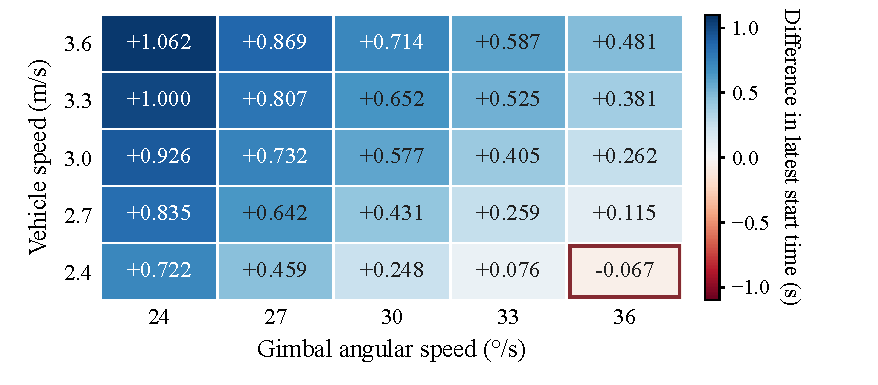
\includegraphics[width=0.93\linewidth]{figures/Sensitivity-Q2-Timing-Heatmap.pdf}
    \caption{Difference in latest start time between the two fixed schedules at an observation duration of \(5\,\mathrm s\). Each cell gives the nearest-assignment baseline value minus the millimeter-coordinate schedule value.}
    \label{fig:q22-sensitivity}
\end{figure}

% 高度临界值由 B5 底面入口的射线参数 u=0.5666189255403465 和屋顶高度计算，站点取毫米方案的 (16.824, 88.760) m。
At the fixed stations and horizontal target coordinates, lowering \(T_3\) from \(55.00\) to \(54.90\,\mathrm m\) caused \(B_5\) to obstruct the sight line from \(V_3\). At \(54.95\,\mathrm m\), the sight line passed \(2.47\,\mathrm{mm}\) above the roof where its horizontal projection entered the building footprint. In this geometry, contact with the roof occurs at \(H_3 \simeq 54.94564\,\mathrm m\). A clear sight line past \(B_5\) requires \(H_3\) to exceed that threshold, corresponding to a decrease of less than approximately \(54.36\,\mathrm{mm}\) from the nominal height.

\subsection{Pointing Reliability and Cumulative Travel Limits}

% 33 个工况及两种角度定义的结果见 results/q3/测向参数敏感性与联合情景_20261122/sensitivity.csv。
For commanded bearing and actual pointing, the projected-normal integrals in Section~\ref{sec:q3-model} give the cumulative travel limit at \(95\%\) coverage and the probability of meeting the \(\pm5^\circ\) tolerance after \(80\,\mathrm m\) of cumulative travel. The initial per-axis localization standard deviation \(a\), localization drift coefficient \(b\), horizontal target range \(D\), and the standard deviations of the gimbal zero-offset and control errors were perturbed individually by \(\pm5\%\), \(\pm10\%\), and \(\pm20\%\). The nominal setting and two joint perturbations brought the total to 33 settings.

The actual-pointing results showed the largest responses to \(D\) and \(b\) over the tested changes. Increasing \(D\) by \(10\%\) extended the travel limit from \(66.837\) to \(75.021\,\mathrm m\). At the prescribed \(D=40\,\mathrm m\), a \(10\%\) reduction in \(b\) lowers the per-axis localization standard deviation at \(80\,\mathrm m\) by \(0.16\,\mathrm m\). An equal relative reduction in \(a\) lowers it by \(0.03\,\mathrm m\). Reductions of \(10\%\) and \(20\%\) in \(b\) alone gave actual-pointing coverage of \(93.71\%\) and \(95.65\%\) at \(80\,\mathrm m\), respectively. With the other parameters at their nominal values, the \(95\%\) boundary corresponds to \(b\leq 0.0167093\,\mathrm{m/m}\), approximately \(16.45\%\) below the nominal coefficient.

At \(80\,\mathrm m\), actual-pointing coverage was \(96.25\%\) under the favorable joint perturbation and \(84.60\%\) under the adverse one (Table~\ref{tab:q3-joint-sensitivity} in \hyperref[app:q3-alternatives]{Appendix~B.4}).

\subsection{Field-Wide Rescheduling under Outage Restrictions}
\label{sec:q4-outage-sensitivity}

The four operating rules were evaluated for field-wide rescheduling (FW) on the same 1,314 outage scenarios, starting from the millimeter-coordinate schedule in Section~\ref{sec:q22-model}. Under the main rule, the original queue is preauthorized, and the original partners may confirm readiness during an outage. The first restriction defers original departures scheduled to begin during the outage. The second defers new synchronized starts until communication recovers. For each rule, schedule replay determined the vehicle states and the alerts already started at recovery.

% FW 四规则取 results/q4/毫米初排与联合断联限制_全程净空四十五厘米_20261121/，主规则仅统计同一批含断联场景。
\begin{table}[!htbp]
    \centering
    \caption{Mean and sample maximum of \(t_{\mathrm{last}}\) for FW over 1,314 matched outage scenarios. The mean assigns equal weight to every scenario.}
    \label{tab:q4-outage-sensitivity}
    \begin{tabular}{@{}lrr@{}}
        \toprule
        Outage rule & Mean (s) & Sample maximum (s) \\
        \midrule
        Main rule & 26.436 & 40.330 \\
        Departure deferral only & 28.230 & 46.108 \\
        Readiness confirmation deferred until recovery & 31.726 & 46.108 \\
        Both restrictions & 32.301 & 46.108 \\
        \bottomrule
    \end{tabular}
\end{table}

In Table~\ref{tab:q4-outage-sensitivity}, deferring readiness confirmation alone increased the mean \(t_{\mathrm{last}}\) by \(5.290\,\mathrm s\). Departure deferral alone increased it by \(1.794\,\mathrm s\). When readiness confirmation was already deferred, adding departure deferral increased the mean by \(0.575\,\mathrm s\). The effect of the departure restriction thus depended on whether the original partners could begin observing during the outage.

Under each rule, all alerts achieved synchronized starts before \(60\,\mathrm s\) in every scenario, yielding \(\eta=1\). All alerts completed five uninterrupted seconds of joint recording by \(60\,\mathrm s\) in 876 scenarios. In the other 438, failure of \(V_3\) or \(V_5\) at \(5\,\mathrm s\) interrupted the joint recording of \(T_1\) after \(3.468\,\mathrm s\). Its synchronized start had already qualified for the score.

\section{Strengths and Weakness}

% OpenCode (Magpie, group/gpt-6.2-sol) assisted with drafting, checking the wording against the reported results, and typesetting this section on 2026-11-22; retain for the team's AI-use report.
% OpenCode（Magpie, group/gpt-6.2-sol）于 2026-11-23 辅助复核和同步队员确认的编号段落，供 AI 使用报告记录。
\subsection{Strengths}

\noindent\hspace*{\parindent}(1)~\textbf{Observable-region analysis} identifies the full optimal arc for \(T_1\). A straight drive of 3.673~m from \(V_4\) attains the shortest feasible travel distance to that arc.
(2)~\textbf{Two-station localization} uses a feasible west--north pair for \(T_2\) to attain the first-order horizontal RMSE bound of 0.143623~m.
(3)~\textbf{Concurrent scheduling} accounts for travel, gimbal motion, and the readiness of both vehicles. Under nominal conditions, the millimeter-coordinate schedule starts the last alert 5.26\% earlier than nearest assignment.
(4)~\textbf{Projected-normal integration} retains the nonlinear bearing geometry and gives the 95\% travel limits for commanded bearing and actual pointing.
(5)~\textbf{Field-wide rescheduling} uses vehicle states at dispatch to reassign pending alerts. Under the main communication rule, all alerts start in 1,751 scenarios with rescheduling and in seven with strict retention.

% 只收紧局限与结论的行距，给两节的同页排版留出空间。
\begingroup
\linespread{1.04}\selectfont
\subsection{Weakness}

\noindent\hspace*{\parindent}(1)~\textbf{Minimum-travel station selection} places the \(T_1\) station at the \(80^\circ\) elevation limit. At that fixed station, the required elevation exceeds the applicable limit in six of the 16 sensitivity tests.
(2)~\textbf{First-order localization RMSE} describes local error around the nominal geometry. Near collinearity, noisy bearings can produce distant intersections or fail to form a valid forward intersection.
(3)~\textbf{Nominal visibility} can be sensitive to target height. With stations and horizontal target coordinates fixed, lowering \(T_3\) by about 54.4~mm brings the sight line from \(V_3\) into contact with the roof of \(B_5\).
(4)~\textbf{Pointing reliability} assumes independent Gaussian errors for a single observation. Using the travel distance and target range in Case~12R, the model estimates an actual-pointing success probability of 84.04\% for \(V_3\) observing \(T_4\).
(5)~\textbf{Rescheduling times} assume zero computation and command-transmission delay. All alerts yield five uninterrupted seconds of joint recording in 1,167 of the 1,751 main-rule scenarios.

% 队员确认的结论讨论稿。样文核对见 research/B题结论写法参考_2025优秀论文.md。
% 初排数值见 results/q2/毫米部署与初排_全程净空四十五厘米_20261121/q22_refinement.csv。
% 重调度数值见 results/q4/毫米初排与联合断联限制_全程净空四十五厘米_20261121/conclusions.md。
\section{Conclusion}

For \(T_1\) and \(T_2\), feasible stations attain the minimum horizontal ranges set by the gimbal elevation limit.
At a fixed bearing intersection angle and noise level, shorter ranges reduce first-order horizontal localization error. With vehicle-position uncertainty and gimbal errors held fixed, however, shorter ranges also lower the probability of meeting the pointing tolerance.
In the nominal three-alert case, coordinating vehicle reuse with travel and gimbal motion advanced the latest joint start by 0.577~s relative to nearest assignment.
Under the main communication rule, field-wide rescheduling started every alert jointly before 60~s in all 1,751 tested scenarios. In 1,167 scenarios, every alert also yielded five uninterrupted seconds of joint recording within the window. In the rest, a vehicle failure interrupted \(T_1\) after its start had counted.
Operational assessments should therefore track pointing reliability and uninterrupted recordings alongside start times. Replay with computation and command transmission delays could test whether interrupted observations can be repeated within 60~s.
\par
\endgroup

% 参考文献独占一页；给两位数编号预留宽度。
\clearpage
\begin{thebibliography}{11}
\bibitem{ref:bearing-geometry}
A. N. Bishop, B. Fidan, B. D. O. Anderson, K. Doğançay, P. N. Pathirana, Optimality analysis of sensor-target localization geometries, Automatica, 46(3):479--492, 2010.

\bibitem{ref:configuration-space}
T. Lozano-Pérez, Spatial Planning: A Configuration Space Approach, IEEE Transactions on Computers, C-32(2):108--120, 1983.

\bibitem{ref:branch-and-bound}
A. H. Land, A. G. Doig, An Automatic Method of Solving Discrete Programming Problems, Econometrica, 28(3):497--520, 1960.

\bibitem{ref:visibility-graph}
T. Lozano-Pérez, M. A. Wesley, An algorithm for planning collision-free paths among polyhedral obstacles, Communications of the ACM, 22(10):560--570, 1979.

\bibitem{ref:sqp}
D. Kraft, Algorithm 733: TOMP--Fortran modules for optimal control calculations, ACM Transactions on Mathematical Software, 20(3):262--281, 1994.

\bibitem{ref:projected-normal}
F. Wang, A. E. Gelfand, Directional data analysis under the general projected normal distribution, Statistical Methodology, 10(1):113--127, 2013.

\bibitem{ref:adaptive-quadrature}
P. Gonnet, A review of error estimation in adaptive quadrature, ACM Computing Surveys, 44(4):1--36, 2012.

\bibitem{ref:brent}
R. P. Brent, An algorithm with guaranteed convergence for finding a zero of a function, The Computer Journal, 14(4):422--425, 1971.

\bibitem{ref:rescheduling}
G. E. Vieira, J. W. Herrmann, E. Lin, Rescheduling Manufacturing Systems: A Framework of Strategies, Policies, and Methods, Journal of Scheduling, 6(1):39--62, 2003.

\bibitem{ref:problem-b-outage}
{\raggedright\urlstyle{same}%
Problem B Author, Clarification on Communication Outage Duration in Problem B, Question 4 (pinned reply), 2026 ShuWei Cup Autumn Competition Q\&A Forum,
\url{https://pd.qq.com/g/pd52619943/post/B_e4b7ff6a0ac20e001441152187121863520X60?subc=745397906}, accessed 2026-11-23.\par}

\bibitem{ref:beam-search}
I. Sabuncuoglu, M. Bayiz, Job shop scheduling with beam search, European Journal of Operational Research, 118(2):390--412, 1999.

\end{thebibliography}

% 组委会《人工智能工具使用规定（2026 年修订）》第 5、6 条：工具入参考文献，报告单页且不计正文限页。
\clearpage
\section*{AI Tool Use Report}
\addcontentsline{toc}{section}{AI Tool Use Report}

We used OpenAI's GPT-6.2 Astra and GPT-6.2 Sol to revise selected sections of the manuscript, improve the presentation of figures, and assist with developing and organizing the accompanying code.

\noindent\textbf{GPT-6.2 Astra (gpt-6.2-astra, OpenAI), 20--23 November 2026.}
We asked the model to polish the English in Sections~4 and~6 and the appendices. It proposed wording changes to selected passages. We adopted selected language edits and made the remaining editorial changes by hand.
For the revised model tests, the tool helped compare the archived checks, expand the English discussion, move the five-vehicle timeline and prepare the Monte Carlo panel and its caption.

\noindent\textbf{GPT-6.2 Sol (gpt-6.2-sol, OpenAI), 20--23 November 2026.}
In the recorded OpenCode sessions, we asked the tool to align the Summary with the main text, apply team feedback to Fig.~\ref{fig:q1-observable-mtdc}, and assemble reproducible materials with solver code, verification scripts, and run instructions. It helped draft and revise passages, refine figures and captions, and implement, check, and organize Python scripts. We incorporated selected wording changes in the Summary, Sections~4 and~6, and the appendices, applied the agreed figure edits, and included the organized code and verification materials in the supporting archive. The team selected the solution variants, reviewed the proposed wording, requested specific removals from Fig.~\ref{fig:q1-observable-mtdc}, and specified the contents of the reproducibility package.

For \hyperref[sec:model-tests]{the model tests}, we asked the tool to organize the existing checks into five subsections that follow the model chapter. The tool proposed English wording for the checks and typeset the discussion draft after team feedback on the structure and paragraph openings.

We are responsible for the submitted manuscript, figures, and code.

% ---------------------开始附录

\clearpage
\endgroup

\section*{Appendix}
% 纸面目录在附录处只显示一级标题，各附录小节仍生成 PDF 书签。
\addcontentsline{toc}{section}{Appendix}
\addtocontents{toc}{\protect\value{tocdepth}=1\relax}

\subsection*{Appendix A. Per-Scenario Dispatch Decisions and Vehicle Timelines}
\label{app:q4}
\addcontentsline{toc}{subsection}{Appendix A. Problem 4 Dispatch Decisions and Vehicle Timelines}

\subsubsection*{A.1 Representative Scores and Dispatch Decisions}

\begin{center}
    \begin{minipage}{\linewidth}
    \centering
    \captionsetup{type=table}
    \caption{Representative scores \((\eta,t_{\rm last})\) for the seven disturbance types. LR denotes local-region rescheduling. A score of 60 s penalizes a missed start. New alerts are given as \((\theta,R)\) with \(H=50\,\mathrm m\). Case 12R repeats Case 12 with both outage restrictions.}
    \label{tab:q4-representative-scores}
    \setlength{\tabcolsep}{4pt}
    \begin{tabular}{@{}l >{\raggedright\arraybackslash}p{0.48\linewidth} ccc@{}}
        \toprule
        Case & Disturbance at 5 s & SR & LR & FW \\
        \midrule
        01 & New alert \((0^\circ,30\,\mathrm m)\) & \((3/4,60)\) & \((1,16.716)\) & \((1,16.716)\) \\
        02 & \(V_1\) fails & \((2/3,60)\) & \((1,11.076)\) & \((1,11.076)\) \\
        03 & \(V_2\) fails & \((2/3,60)\) & \((1,10.830)\) & \((1,10.830)\) \\
        04 & \(V_3\) fails & \((2/3,60)\) & \((1,10.830)\) & \((1,10.830)\) \\
        05 & \(V_4\) fails & \((2/3,60)\) & \((1,11.076)\) & \((1,11.076)\) \\
        06 & \(V_5\) fails & \((1,10.392)\) & \((1,10.392)\) & \((1,10.392)\) \\
        07 & Outage with recovery at 30 s & \((1,10.392)\) & \((1,10.392)\) & \((1,10.392)\) \\
        08 & New alert \((90^\circ,40\,\mathrm m)\) and \(V_1\) failure & \((1/2,60)\) & \((1,23.136)\) & \((1,23.186)\) \\
        09 & New alert \((270^\circ,50\,\mathrm m)\) and recovery at 10 s & \((3/4,60)\) & \((1,16.716)\) & \((1,16.716)\) \\
        10 & \(V_2\) failure and recovery at 10 s & \((2/3,60)\) & \((1,12.766)\) & \((1,12.766)\) \\
        11 & New alert \((240^\circ,40\,\mathrm m)\), \(V_5\) failure, recovery at 20~s & \((3/4,60)\) & \((1,26.121)\) & \((1,23.836)\) \\
        12 & New alert \((135^\circ,50\,\mathrm m)\), \(V_1\) failure, recovery at 30~s & \((1/2,60)\) & \((1,41.718)\) & \((1,40.330)\) \\
        12R & Case 12 with both outage restrictions & \((1/2,60)\) & \((1,47.495)\) & \((1,46.108)\) \\
        \bottomrule
    \end{tabular}
    \end{minipage}
\end{center}

The original assignments are $T_1:(\mathrm{3F},\mathrm{5E})$, $T_2:(\mathrm{1A},\mathrm{4G})$, and $T_3:(\mathrm{2B},\mathrm{3H})$. For example, 3F means vehicle $V_3$ at station F in Table~\ref{tab:q4-sites}. Table~\ref{tab:q4-representative-scores} defines the cases. Table~\ref{tab:q4-dispatch} lists the vehicle--station assignments for alerts pending at dispatch. Locked alerts retain the original assignments. SR also retains them for pending alerts, and its column identifies the alerts that do not start. The order and timing of the assignments are given in A.3 and A.4. Table~\ref{tab:q4-controls} gives the assignments and scores for two controls defined in \hyperref[app:q4-alternatives]{Appendix~B.5}.

\begingroup
\setlength{\tabcolsep}{4pt}
\begin{longtable}{@{}l >{\raggedright\arraybackslash}p{0.14\linewidth}
    >{\raggedright\arraybackslash}p{0.12\linewidth}
    >{\raggedright\arraybackslash}p{0.29\linewidth}
    >{\raggedright\arraybackslash}p{0.29\linewidth}@{}}
    \caption{Vehicle--station assignments for pending alerts.}\label{tab:q4-dispatch}\\
    \toprule
    Case & Locked at dispatch & Missed by SR & LR assignments & FW assignments \\
    \midrule
    \endfirsthead
    \toprule
    Case & Locked at dispatch & Missed by SR & LR assignments & FW assignments \\
    \midrule
    \endhead
    \midrule
    \multicolumn{5}{r@{}}{\emph{Continued on the next page}} \\
    \endfoot
    \bottomrule
    \endlastfoot
    01 & $T_1$ & $T_4$ & $T_2$:~1A,~4G; $T_3$:~1A,~2B; $T_4$:~3F,~5I & $T_2$:~1A,~4G; $T_3$:~1A,~2J; $T_4$:~3C,~5K \\
    02 & $T_1$ & $T_2$ & $T_2$:~3F,~4G; $T_3$:~2B,~5E & $T_2$:~3F,~4G; $T_3$:~2B,~5E \\
    03 & $T_1$ & $T_3$ & $T_2$:~1A,~4G; $T_3$:~3H,~5E & $T_2$:~1A,~4G; $T_3$:~3L,~5E \\
    04 & $T_1$ & $T_3$ & $T_2$:~1A,~4G; $T_3$:~2B,~5E & $T_2$:~1A,~4G; $T_3$:~2B,~5E \\
    05 & $T_1$ & $T_2$ & $T_2$:~1A,~3F; $T_3$:~2B,~5E & $T_2$:~1A,~3F; $T_3$:~2B,~5E \\
    06 & $T_1$ & None & $T_2$:~1A,~4G; $T_3$:~2B,~3H & $T_2$:~1A,~4G; $T_3$:~2B,~3H \\
    07 & $T_1,T_2,T_3$ & None & No pending alert & No pending alert \\
    08 & $T_1$ & $T_2,T_4$ & $T_2$:~2M,~4G; $T_3$:~3H,~5I; $T_4$:~3F,~5I & $T_2$:~2N,~4G; $T_3$:~3H,~5I; $T_4$:~3F,~5O \\
    09 & $T_1,T_2$ & $T_4$ & $T_3$:~1A,~2B; $T_4$:~3P,~5Q & $T_3$:~1A,~3L; $T_4$:~2B,~5R \\
    10 & $T_1,T_2$ & $T_3$ & $T_3$:~3H,~5E & $T_3$:~3H,~5E \\
    11 & $T_1,T_2,T_3$ & $T_4$ & $T_4$:~1A,~3V & $T_4$:~1S,~3U \\
    12 & $T_1,T_3$ & $T_2,T_4$ & $T_2$:~2M,~4G; $T_4$:~3W,~5E & $T_2$:~2N,~5Y; $T_4$:~3X,~4G \\
    12R & $T_1$ & $T_2,T_4$ & $T_2$:~2M,~5E; $T_3$:~3H,~5E; $T_4$:~3W,~4G & $T_2$:~2N,~5E; $T_3$:~3H,~5E; $T_4$:~3X,~4G \\
\end{longtable}
\endgroup

\begin{center}
    \begin{minipage}{\linewidth}
    \centering
    \captionsetup{type=table}
    \caption{Additional policy controls for cases discussed in Section~\ref{sec:q4-dispatch-effects}.}
    \label{tab:q4-controls}
    \begin{tabular}{@{}lllr@{}}
        \toprule
        Case & Control & Pending assignment & Score $(\eta,t_{\rm last})$ \\
        \midrule
        10 & Fixed stations (FS) & $T_3$:~3H,~4B & $(1,43.965896)$ \\
        11 & Retain and append (RA) & $T_4$:~1T,~3U & $(1,23.836399)$ \\
        \bottomrule
    \end{tabular}
    \end{minipage}
\end{center}

\subsubsection*{A.2 Station Coordinates}

Stations A--E are the initial positions of $V_1$--$V_5$, respectively. Coordinates are in meters. Rescheduled coordinates are rounded here for display.

\begin{center}
    \begin{minipage}{\linewidth}
    \centering
    \captionsetup{type=table}
    \caption{Station coordinates used in the representative scenarios.}
    \label{tab:q4-sites}
    \begin{tabular}{@{}cl@{\hspace{1.5em}}cl@{\hspace{1.5em}}cl@{}}
        \toprule
        Site & $(x,y)$ (m) & Site & $(x,y)$ (m) & Site & $(x,y)$ (m) \\
        \midrule
        A & $(15,14)$         & J & $(87.333333,7.666667)$   & S & $(12,12)$ \\
        B & $(88,10)$         & K & $(49.750,96.250)$       & T & $(12.500,11.500)$ \\
        C & $(14,86)$         & L & $(16.250,89.750)$       & U & $(16.500,92.250)$ \\
        D & $(88,68)$         & M & $(66,7.666667)$         & V & $(20.666667,98)$ \\
        E & $(50,93)$         & N & $(71.750,2.500)$        & W & $(11.333333,98)$ \\
        F & $(15.033,87.088)$ & O & $(46.761084,97.819436)$ & X & $(12.993476,93.656408)$ \\
        G & $(88.064,70.901)$ & P & $(20.666667,91.200)$    & Y & $(49.250,93.250)$ \\
        H & $(16.824,88.760)$ & Q & $(56.666667,92)$        &   & \\
        I & $(46.333333,98)$  & R & $(52.500,93.250)$       &   & \\
        \bottomrule
    \end{tabular}
    \end{minipage}
\end{center}

\subsubsection*{A.3 Common Initial Timeline and Scenario Index}

The common starting plan is the millimeter deployment in Table~\ref{tab:q22-millimeter}. Read each vehicle's timeline up to $5\,\mathrm{s}$ in Table~\ref{tab:q4-prefix}, then use Table~\ref{tab:q4-index} to find its continuation in Table~\ref{tab:q4-continuations}. Every continuation begins at $5\,\mathrm{s}$. Later times are absolute event times in seconds. An unchanged phase across the join continues without interruption. Each phase ends at the next recorded time, and the final phase ends at $60\,\mathrm{s}$.

\texttt{D} means driving, \texttt{P} pointing, \texttt{W} waiting at the station after pointing, \texttt{O} observing, \texttt{R} resetting after observation, \texttt{X} resetting after cancellation, \texttt{I} parked idle, and \texttt{F} withdrawn from service. For example, D3$\to$H means departure toward station H for $T_3$, with arrival at the end of that phase. All recorded drives in these cases are straight segments. An observation is joint only while the two assigned vehicles' \texttt{O} intervals overlap. A final \texttt{W} means the vehicle waits to $60\,\mathrm{s}$ without starting that observation.

\begin{center}
    \begin{minipage}{\linewidth}
    \centering
    \captionsetup{type=table}
    \caption{Common initial timeline over $[0,5)\,\mathrm{s}$.}
    \label{tab:q4-prefix}
    \begin{tabular}{@{}llp{0.60\linewidth}@{}}
        \toprule
        Vehicle & Initial station & Phase starts (s) \\
        \midrule
        $V_1$ & A & P2~0; W2~3.129448 \\
        $V_2$ & B & P3~0 \\
        $V_3$ & C & D1$\to$F~0; P1~0.500093; O1~1.532122 \\
        $V_4$ & D & D2$\to$G~0; P2~0.967235 \\
        $V_5$ & E & P1~0; W1~1.532033; O1~1.532122 \\
        \bottomrule
    \end{tabular}
    \end{minipage}
\end{center}

When multiple policies share a row in Table~\ref{tab:q4-index}, all five displayed timelines coincide.

\begin{longtable}{@{}llccccc@{}}
    \caption{Five-vehicle continuation index by scenario and policy.}\label{tab:q4-index}\\
    \toprule
    Case & Policy & $V_1$ & $V_2$ & $V_3$ & $V_4$ & $V_5$ \\
    \midrule
    \endfirsthead
    \toprule
    Case & Policy & $V_1$ & $V_2$ & $V_3$ & $V_4$ & $V_5$ \\
    \midrule
    \endhead
    \midrule
    \multicolumn{7}{r@{}}{\emph{Continued on the next page}} \\
    \endfoot
    \bottomrule
    \endlastfoot
    01 & SR & 1a & 2a & 3a & 4a & 5a \\*
    01 & LR & 1b & 2b & 3b & 4a & 5b \\*
    01 & FW & 1b & 2c & 3c & 4a & 5c \\
    02 & SR & 1c & 2a & 3a & 4b & 5a \\*
    02 & LR / FW & 1c & 2d & 3d & 4c & 5d \\
    03 & SR & 1a & 2e & 3e & 4a & 5a \\*
    03 & LR & 1a & 2e & 3f & 4a & 5d \\*
    03 & FW & 1a & 2e & 3g & 4a & 5d \\
    04 & SR & 1a & 2f & 3h & 4a & 5a \\*
    04 & LR / FW & 1a & 2d & 3h & 4a & 5d \\
    05 & SR & 1d & 2a & 3a & 4d & 5a \\*
    05 & LR / FW & 1e & 2d & 3d & 4d & 5d \\
    06 & SR / LR / FW & 1a & 2a & 3a & 4a & 5e \\
    07 & SR / LR / FW & 1a & 2a & 3a & 4a & 5a \\
    08 & SR & 1c & 2a & 3a & 4b & 5a \\*
    08 & LR & 1c & 2g & 3i & 4e & 5f \\*
    08 & FW & 1c & 2h & 3j & 4f & 5g \\
    09 & SR & 1a & 2a & 3a & 4a & 5a \\*
    09 & LR & 1b & 2b & 3k & 4a & 5h \\*
    09 & FW & 1b & 2i & 3l & 4a & 5i \\
    10 & SR & 1a & 2e & 3e & 4a & 5a \\*
    10 & LR / FW & 1a & 2e & 3m & 4a & 5j \\*
    10 & FS & 1a & 2e & 3n & 4g & 5a \\
    11 & SR & 1a & 2a & 3a & 4a & 5e \\*
    11 & LR & 1f & 2a & 3o & 4a & 5e \\*
    11 & FW & 1g & 2a & 3p & 4a & 5e \\*
    11 & RA & 1h & 2a & 3p & 4a & 5e \\
    12 & SR & 1c & 2a & 3a & 4b & 5a \\*
    12 & LR & 1c & 2j & 3q & 4h & 5k \\*
    12 & FW & 1c & 2k & 3r & 4i & 5l \\
    12R & SR & 1c & 2l & 3s & 4b & 5a \\*
    12R & LR & 1c & 2m & 3t & 4j & 5m \\*
    12R & FW & 1c & 2n & 3u & 4k & 5n \\
\end{longtable}

For example, in Case 10 under LR or FW, $V_3$ follows continuation 3m: it completes $T_1$, transfers to H, finishes pointing at $10.391510\,\mathrm{s}$, and waits until $V_5$ is ready at $12.765521\,\mathrm{s}$. Under SR, continuation 3e ends in \texttt{W3}, so $V_3$ waits at H through $60\,\mathrm{s}$ and does not start $T_3$.

\subsubsection*{A.4 Vehicle Continuations on $[5,60]\,\mathrm{s}$}

\begin{longtable}{@{}l >{\raggedright\arraybackslash}p{0.91\linewidth}@{}}
    \caption{Vehicle continuations from $5\,\mathrm{s}$ to $60\,\mathrm{s}$.}\label{tab:q4-continuations}\\
    \toprule
    ID & Phase sequence; first phase begins at $5\,\mathrm{s}$ \\
    \midrule
    \endfirsthead
    \toprule
    ID & Phase sequence; first phase begins at $5\,\mathrm{s}$ \\
    \midrule
    \endhead
    \midrule
    \multicolumn{2}{r@{}}{\emph{Continued on the next page}} \\
    \endfoot
    \bottomrule
    \endlastfoot
    \multicolumn{2}{@{}l}{\textbf{Vehicle $V_1$}} \\*
    1a & W2; O2~6.927598; R2~11.927598; I~15.057046 \\
    1b & W2; O2~6.927598; R2~11.927598; P3~15.057046; O3~16.715950; R3~21.715950; I~23.374853 \\
    1c & F \\
    1d & W2 \\
    1e & W2; O2~11.075774; R2~16.075774; I~19.205222 \\
    1f & W2; O2~6.927598; R2~11.927598; I~15.057046; P4~20; W4~22.419306; O4~26.120941; R4~31.120941; I~33.540248 \\
    1g & W2; O2~6.927598; R2~11.927598; I~15.057046; D4$\to$S~20; P4~21.201850; W4~23.505833; O4~23.836399; R4~28.836399; I~31.140381 \\
    1h & W2; O2~6.927598; R2~11.927598; I~15.057046; D4$\to$T~20; P4~21.178511; W4~23.496087; O4~23.836399; R4~28.836399; I~31.153975 \\
    \addlinespace
    \multicolumn{2}{@{}l}{\textbf{Vehicle $V_2$}} \\*
    2a & P3; W3~5.777589; O3~10.391510; R3~15.391510; I~21.169099 \\
    2b & P3; W3~5.777589; O3~16.715950; R3~21.715950; I~27.493539 \\
    2c & X; D3$\to$J~10; P3~10.808901; W3~16.423329; O3~16.715950; R3~21.715950; I~27.330377 \\
    2d & P3; W3~5.777589; O3~10.829675; R3~15.829675; I~21.607265 \\
    2e & F \\
    2f & P3; W3~5.777589 \\
    2g & X; D2$\to$M~10; P2~17.374464; O2~21.717600; R2~26.717600; I~31.060736 \\
    2h & X; D2$\to$N~10; P2~15.965759; O2~20.330420; R2~25.330420; I~29.695081 \\
    2i & P3; W3~5.777589; P4~10; W4~10.713863; O4~13.888680; R4~18.888680; I~24.397228 \\
    2j & P3; W3~5.777589; O3~10.391510; R3~15.391510; I~21.169099; D2$\to$M~30; P2~37.374464; O2~41.717600; R2~46.717600; I~51.060736 \\
    2k & P3; W3~5.777589; O3~10.391510; R3~15.391510; I~21.169099; D2$\to$N~30; P2~35.965759; O2~40.330420; R2~45.330420; I~49.695081 \\
    2l & P3; W3~5.777589; O3~32.827358; R3~37.827358; I~43.604947 \\
    2m & P3; W3~5.777589; X~30; D2$\to$M~35.777589; P2~43.152053; O2~47.495189; R2~52.495189; I~56.838325 \\
    2n & P3; W3~5.777589; X~30; D2$\to$N~35.777589; P2~41.743348; O2~46.108009; R2~51.108009; I~55.472671 \\
    \addlinespace
    \multicolumn{2}{@{}l}{\textbf{Vehicle $V_3$}} \\*
    3a & O1; R1~6.532122; D3$\to$H~7.564152; P3~8.380871; O3~10.391510; R3~15.391510; I~17.402149 \\
    3b & O1; R1~6.532122; P4~7.564152; W4~8.653684; O4~11.962761; R4~16.962761; I~18.052294 \\
    3c & O1; R1~6.532122; D4$\to$C~7.564152; P4~8.064245; W4~9.149478; O4~11.044460; R4~16.044460; I~17.129693 \\
    3d & O1; R1~6.532122; P2~7.564152; O2~11.075774; R2~16.075774; I~19.587396 \\
    3e & O1; R1~6.532122; D3$\to$H~7.564152; P3~8.380871; W3~10.391510 \\
    3f & O1; R1~6.532122; D3$\to$H~7.564152; P3~8.380871; W3~10.391510; O3~10.829675; R3~15.829675; I~17.840314 \\
    3g & O1; R1~6.532122; D3$\to$L~7.564152; P3~8.539819; W3~10.550274; O3~10.829675; R3~15.829675; I~17.840131 \\
    3h & F \\
    3i & O1; R1~6.532122; P4~7.564152; W4~9.358591; O4~12.784636; R4~17.784636; D3$\to$H~19.579075; P3~20.395794; W3~22.406433; O3~23.136444; R3~28.136444; I~30.147083 \\
    3j & O1; R1~6.532122; P4~7.564152; W4~9.358591; O4~12.666382; R4~17.666382; D3$\to$H~19.460820; P3~20.277539; W3~22.288178; O3~23.185928; R3~28.185928; I~30.196567 \\
    3k & O1; R1~6.532122; D3$\to$H~7.564152; P3~8.380871; X~10; D4$\to$P~11.619129; P4~13.136425; O4~15.542101; R4~20.542101; I~22.947776 \\
    3l & O1; R1~6.532122; D3$\to$H~7.564152; P3~8.380871; X~10; D3$\to$L~11.619129; P3~12.000585; W3~14.011040; O3~16.715950; R3~21.715950; I~23.726405 \\
    3m & O1; R1~6.532122; D3$\to$H~7.564152; P3~8.380871; W3~10.391510; O3~12.765521; R3~17.765521; I~19.776159 \\
    3n & O1; R1~6.532122; D3$\to$H~7.564152; P3~8.380871; W3~10.391510; O3~43.965896; R3~48.965896; I~50.976535 \\
    3o & O1; R1~6.532122; D3$\to$H~7.564152; P3~8.380871; O3~10.391510; R3~15.391510; I~17.402149; D4$\to$V~20; P4~23.335727; O4~26.120941; R4~31.120941; I~33.906155 \\
    3p & O1; R1~6.532122; D3$\to$H~7.564152; P3~8.380871; O3~10.391510; R3~15.391510; I~17.402149; D4$\to$U~20; P4~21.168336; O4~23.836399; R4~28.836399; I~31.504462 \\
    3q & O1; R1~6.532122; D3$\to$H~7.564152; P3~8.380871; O3~10.391510; R3~15.391510; I~17.402149; D4$\to$W~30; P4~33.582752; O4~36.093591; R4~41.093591; I~43.604430 \\
    3r & O1; R1~6.532122; D3$\to$H~7.564152; P3~8.380871; O3~10.391510; R3~15.391510; I~17.402149; D4$\to$X~30; P4~32.072243; O4~34.738910; R4~39.738910; I~42.405576 \\
    3s & O1; R1~6.532122; I~7.564152; D3$\to$H~30; P3~30.816719; O3~32.827358; R3~37.827358; I~39.837997 \\
    3t & O1; R1~6.532122; I~7.564152; D3$\to$H~30; P3~30.816719; O3~32.827358; R3~37.827358; D4$\to$W~39.837997; P4~43.420749; O4~45.931588; R4~50.931588; I~53.442427 \\
    3u & O1; R1~6.532122; I~7.564152; D3$\to$H~30; P3~30.816719; O3~32.827358; R3~37.827358; D4$\to$X~39.837997; P4~41.910240; O4~44.576906; R4~49.576906; I~52.243573 \\
    \addlinespace
    \multicolumn{2}{@{}l}{\textbf{Vehicle $V_4$}} \\*
    4a & P2; O2~6.927598; R2~11.927598; I~17.887962 \\
    4b & P2; W2~6.927598 \\
    4c & P2; W2~6.927598; O2~11.075774; R2~16.075774; I~22.036137 \\
    4d & F \\
    4e & P2; W2~6.927598; O2~21.717600; R2~26.717600; I~32.677963 \\
    4f & P2; W2~6.927598; O2~20.330420; R2~25.330420; I~31.290783 \\
    4g & P2; O2~6.927598; R2~11.927598; D3$\to$B~17.887962; P3~38.188306; O3~43.965896; R3~48.965896; I~54.743485 \\
    4h & P2; W2~6.927598; O2~41.717600; R2~46.717600; I~52.677963 \\
    4i & P2; W2~6.927598; P4~30; W4~30.331616; O4~34.738910; R4~39.738910; I~45.367657 \\
    4j & P2; W2~6.927598; X~30; P4~35.960363; W4~41.589110; O4~45.931588; R4~50.931588; I~56.560335 \\
    4k & P2; W2~6.927598; P4~30; W4~30.331616; O4~44.576906; R4~49.576906; I~55.205653 \\
    \addlinespace
    \multicolumn{2}{@{}l}{\textbf{Vehicle $V_5$}} \\*
    5a & O1; R1~6.532122; I~8.064155 \\
    5b & O1; R1~6.532122; D4$\to$I~8.064155; P4~10.130941; O4~11.962761; R4~16.962761; I~18.794582 \\
    5c & O1; R1~6.532122; D4$\to$K~8.064155; P4~9.150689; O4~11.044460; R4~16.044460; I~17.938232 \\
    5d & O1; R1~6.532122; P3~8.064155; O3~10.829675; R3~15.829675; I~18.595196 \\
    5e & F \\
    5f & O1; R1~6.532122; D4$\to$I~8.064155; P4~10.130941; O4~12.784636; R4~17.784636; P3~20.438331; O3~23.136444; R3~28.136444; I~30.834557 \\
    5g & O1; R1~6.532122; D4$\to$O~8.064155; P4~9.999715; O4~12.666382; R4~17.666382; D3$\to$I~20.333048; P3~20.487815; O3~23.185928; R3~28.185928; I~30.884041 \\
    5h & O1; R1~6.532122; I~8.064155; D4$\to$Q~10; P4~12.247083; W4~15.385237; O4~15.542101; R4~20.542101; I~23.680255 \\
    5i & O1; R1~6.532122; I~8.064155; D4$\to$R~10; P4~10.837490; O4~13.888680; R4~18.888680; I~21.939870 \\
    5j & O1; R1~6.532122; I~8.064155; P3~10; O3~12.765521; R3~17.765521; I~20.531041 \\
    5k & O1; R1~6.532122; I~8.064155; P4~30; W4~35.593304; O4~36.093591; R4~41.093591; I~46.686895 \\
    5l & O1; R1~6.532122; I~8.064155; D2$\to$Y~30; P2~30.263523; W2~35.313615; O2~40.330420; R2~45.330420; I~50.380512 \\
    5m & O1; R1~6.532122; I~8.064155; P3~30; W3~32.765521; O3~32.827358; R3~37.827358; P2~40.592878; W2~45.668021; O2~47.495189; R2~52.495189; I~57.570331 \\
    5n & O1; R1~6.532122; I~8.064155; P3~30; W3~32.765521; O3~32.827358; R3~37.827358; P2~40.592878; W2~45.668021; O2~46.108009; R2~51.108009; I~56.183152 \\
\end{longtable}

\clearpage
\subsection*{Appendix B. Alternative Methods and Independent Checks}
\label{app:alternatives}
\addcontentsline{toc}{subsection}{Appendix B. Alternative Methods and Independent Checks}

% 最大最小净空与独立复核：results/q1/可观测区域与最优站位_连续圆弧_20261120/。
\subsubsection*{B.1 Maximum Minimum Clearance and Projected Station Search}
\label{app:q1-alternatives}

The maximum minimum clearance criterion (MMCC) selects a quality-optimal station with the greatest minimum distance from the vehicle body to buildings and the field boundary. For \(p=(x,y)\), the secondary problem is
\begin{equation}
\label{eq:q1-mmcc-objective}
\begin{aligned}
&\max_{p\in\mathcal A_1:\,r_1(p)=r^*} c(p),\\
&c(p)=\min\!\left\{x-1.5,\,98.5-x,\,y-1.5,\,98.5-y,\,
      \min_j\bigl[\operatorname{dist}(p,F_j)-1.5\bigr]\right\}.
\end{aligned}
\end{equation}
The eastern field boundary and the northeast corner of \(B_2\) impose the two active limits on clearance. Equating the two distances on the optimal arc gives a station at \(\varphi\simeq56.503855631^\circ\), or \((88.825410107,76.322854075)\,\mathrm m\), with minimum clearance \(9.674589893\,\mathrm m\). An upper bound based on these distances and interval subdivision of the arc differs from the achieved clearance by less than \(10^{-8}\,\mathrm m\). The station retains the same \(Q^*\) and \(80^\circ\) elevation as the MTDC station. The reported coordinates are display values because inward rounding can violate the elevation limit.

\begin{figure}[!htbp]
    \centering
    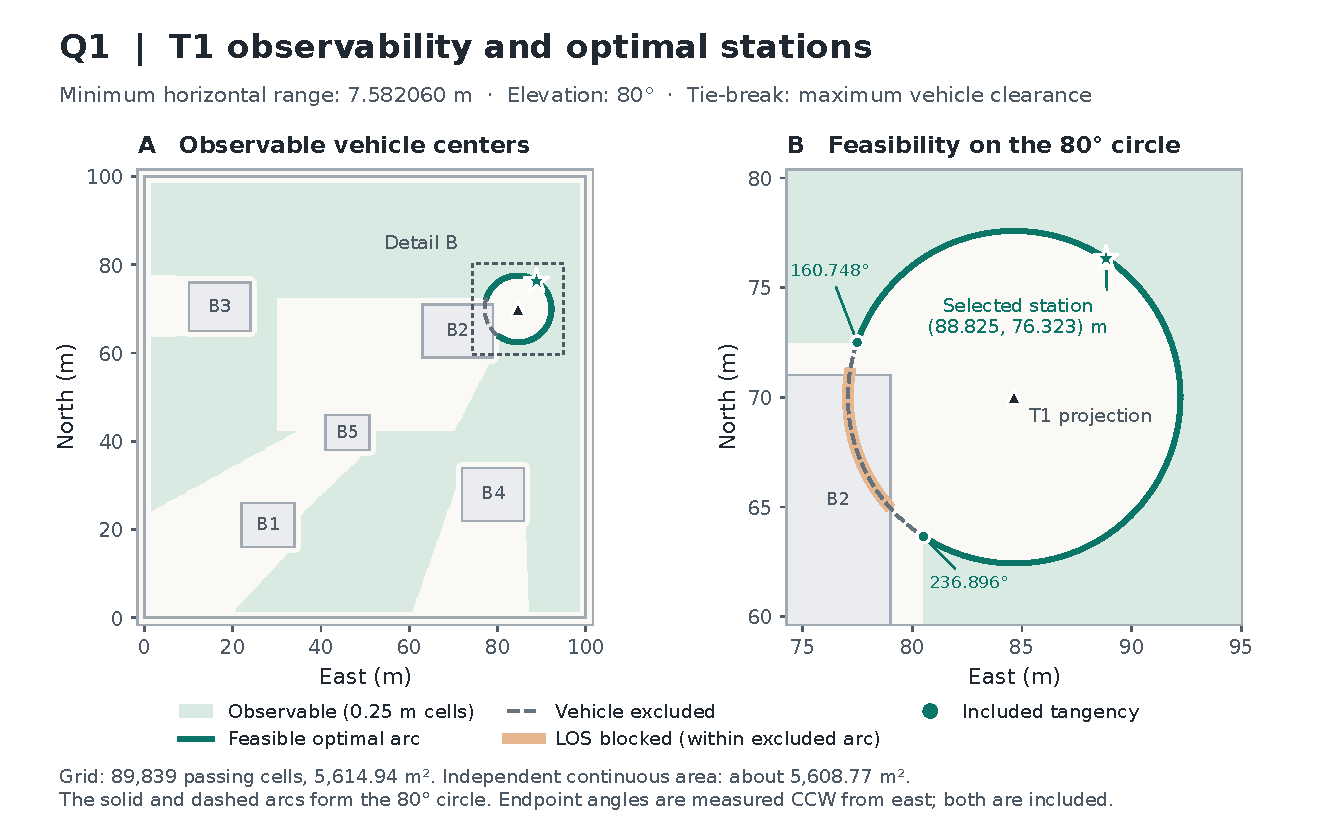
\includegraphics[width=\linewidth]{figures/Q1-Maximum-Clearance.pdf}
    \caption{The maximum minimum clearance station on the optimal arc for \(T_1\). The star marks the MMCC solution. Shading uses 0.25 m cells.}
    \label{fig:q1-observable-mmcc}
\end{figure}

An independent optimization first minimizes squared range in the station plane. In a second stage, it maximizes \(c(p)\) at that range. Starting from 49 initial points, 36 first-stage results passed the three-dimensional feasibility check, as did all 35 second-stage results. The calculation recovered the optimal range and located the MMCC station within \(1.3\times10^{-8}\,\mathrm m\) of the solution in Fig.~\ref{fig:q1-observable-mmcc}. On the 0.5, 0.25 and 0.125 m grids, projected and direct three-dimensional calculations give identical results at every tested center. The vertical-strip bounds on the continuous area are \(5608.767083\) and \(5608.774146\,\mathrm{m^2}\), consistent with the estimate in Section~\ref{sec:q1-model}.

% MMCC 的扰动站点、原站仰角与可观测面积见 results/q1/仰角目标位置与净空敏感性_20261122/。
Under the one-factor perturbations in Section~\ref{sec:q1-sensitivity}, the maximum minimum clearance criterion was reapplied to the quality-maximizing stations. At an elevation limit of \(79^\circ\), the reselected station lay \(1.120\,\mathrm m\) from the nominal station, and its minimum vehicle-body clearance increased from \(9.675\) to \(9.976\,\mathrm m\). With the nominal MMCC station held fixed, an elevation violation occurred in six settings. These were the two reductions in the elevation limit, the two increases in target height, and the \(0.5\,\mathrm m\) shifts of \(T_1\) to the east and to the north (Fig.~\ref{fig:q1-sensitivity}).

\begin{figure}[!htbp]
    \centering
    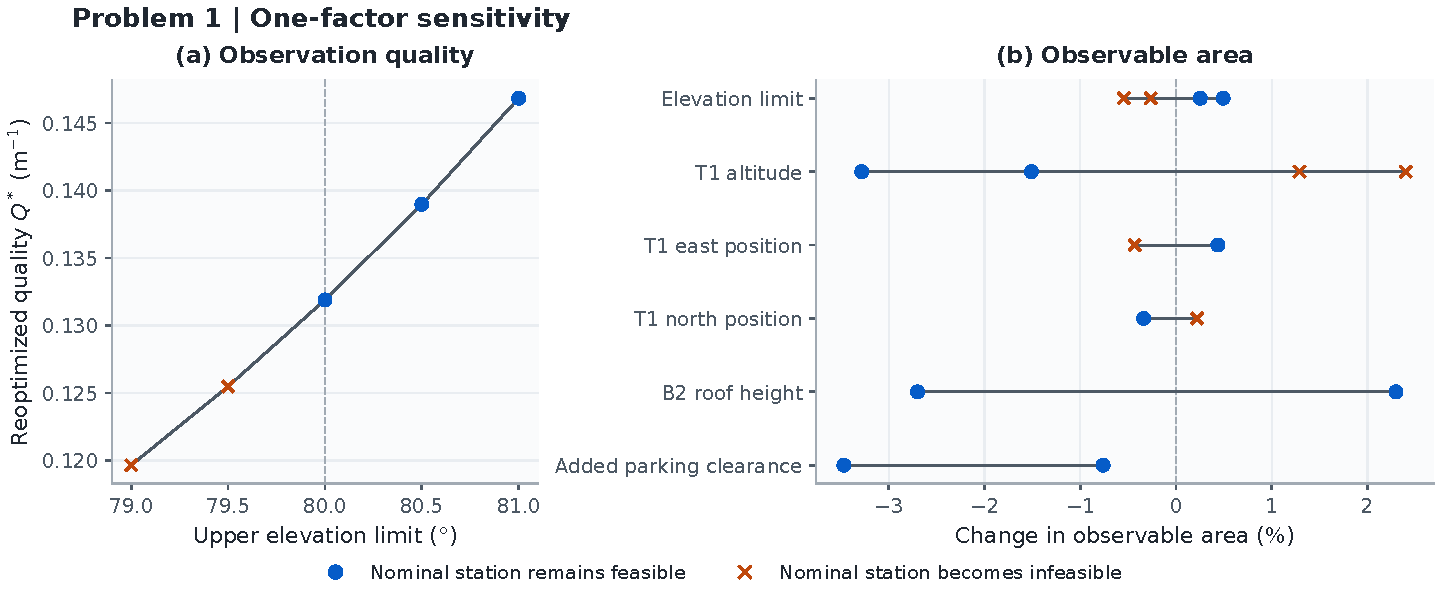
\includegraphics[width=\linewidth]{figures/Sensitivity-Q1.pdf}
    \caption{Maximum observation quality after station reselection at each elevation limit (a) and relative changes in observable area across the one-factor tests (b). Crosses identify perturbations for which the nominal MMCC station violates the elevation constraint.}
    \label{fig:q1-sensitivity}
\end{figure}

% 等精度对照：results/q2/双站等精度两方案对照_20261122/two_schemes.csv。
% 毫米部署：results/q2/毫米部署与初排_全程净空四十五厘米_20261121/q21_practical.json。
\subsubsection*{B.2 Alternative Equal-Accuracy Pairs and Millimeter Deployment}
\label{app:q21-alternatives}

Every observable orthogonal pair on the \(r_0\) circle attains the first-order RMSE bound in Section~\ref{sec:q21-model}, provided two vehicles can reach the stations. The grid construction screens feasible vehicle--station combinations at \(0.25^\circ\) increments. It then uses a \(10^\circ\) representative grid and a \(0.10\,\mathrm m\) parking-clearance filter to find the pair with the shortest total drive on that grid. The selected routes also pass the independent \(0.45\,\mathrm m\) clearance check.

The clearance-binding construction minimizes the longer drive within the equal-accuracy family with \(0.45\,\mathrm m\) of body clearance. The straight-line times for \(V_1,V_2,V_4\) to reach the range circle are bounded below by \(17.605\), \(31.111\) and \(23.761\,\mathrm s\), respectively. A pair reaching both stations within \(13.294\,\mathrm s\) must therefore use \(V_3,V_5\). On the northeastern approach arc for \(V_5\), clearing the roof of \(B_3\) requires \(y>77.521739\,\mathrm m\), and the body clearance requires \(y\ge77.95\,\mathrm m\). Let \(q\) be the intersection of this clearance line with the northeastern arc. The points on the circle closer to the origin of \(V_5\) than \(q\) all lie below that line and within \(1.95\,\mathrm m\) of the footprint of \(B_3\). The straight drive to \(q\) thus gives \(13.293759977\,\mathrm s\) as a lower bound on the longer drive in any equal-accuracy pair.

With \(d=5.4500002\,\mathrm m\) and \(a_c=\sqrt{r_0^2-d^2}\), the construction places \(V_3\) at \(T'_2+(-d,a_c)\) and \(V_5\) at \(T'_2+(a_c,d)\). Both routes are straight, and the longer drive lies within \(1.4\times10^{-7}\,\mathrm s\) of its lower bound. Both constructions have an \(8.229012\,\mathrm m\) baseline, a \(90^\circ\) intersection and a \(0.143623358\,\mathrm m\) first-order RMSE. The clearance-binding pair shortens the longer drive by 12.709 ms and total travel by 87.753 mm relative to the grid pair, whose \(V_5\) station has more clearance from \(B_3\).

\begin{table}[!htbp]
    \centering
    \caption{Alternative equal-accuracy constructions for \(T_2\). Coordinates are rounded for display.}
    \label{tab:q21-schemes}
    \begin{tabular}{@{}lrr@{}}
        \toprule
        Indicator & Grid construction & \shortstack[r]{Clearance-binding\\construction} \\
        \midrule
        \(V_3\) station (m) & \((5.560982,74.490144)\) & \((5.578857,74.538583)\) \\
        \(V_5\) station (m) & \((13.019000,77.967874)\) & \((13.067439,77.950000)\) \\
        \(V_3\) drive time (s) & 4.757378 & 4.740836 \\
        \(V_5\) drive time (s) & 13.306469 & 13.293760 \\
        Total path length (m) & 54.191542 & 54.103789 \\
        \(V_5\) body clearance to \(B_3\) (m) & 0.467874 & 0.450000 \\
        \bottomrule
    \end{tabular}
\end{table}

\begin{figure}[!htbp]
    \centering
    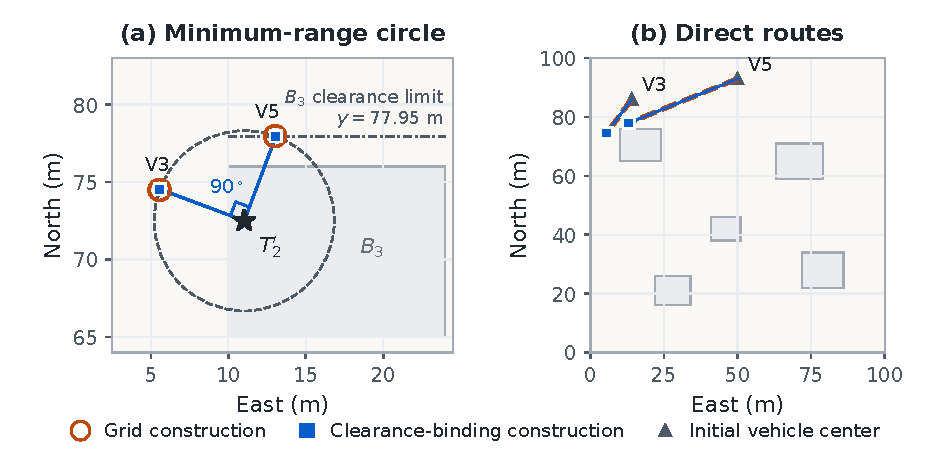
\includegraphics[width=\linewidth]{figures/Q21-Station-Pairs.pdf}
    \caption{Grid and clearance-binding station pairs on the minimum-range circle (left) and their straight routes (right).}
    \label{fig:q21-schemes}
\end{figure}

Table~\ref{tab:q21-schemes} and Fig.~\ref{fig:q21-schemes} compare the two exact constructions. Directly rounding the clearance-binding \(V_5\) station to \((13.067,77.950)\,\mathrm m\) raises its elevation to \(80.000260^\circ\). Shifting both stations radially outward by \((0.10+0.0005\sqrt{2})\,\mathrm m\) before rounding leaves at least \(0.10\,\mathrm m\) of radial margin after coordinate rounding. The resulting stations \((5.485,74.574)\,\mathrm m\) for \(V_3\) and \((13.103,78.044)\,\mathrm m\) for \(V_5\) were verified at those coordinates. The straight drives take \(4.749956\) and \(13.270981\,\mathrm s\), with a minimum building clearance of \(0.544\,\mathrm m\) over the two routes and a minimum elevation margin of about \(0.169^\circ\). The baseline is \(8.371071\,\mathrm m\), the intersection angle is \(90.000812^\circ\), and the first-order RMSE increases to \(0.146101709\,\mathrm m\).

% 噪声响应底表见 results/q2/毫米部署与初排敏感性_20261122/q21_noise_sensitivity.csv。
At fixed geometry, the first-order horizontal RMSE varies linearly with the common bearing-error standard deviation. The two exact orthogonal constructions have equal ranges and give the same RMSE throughout the scan in Table~\ref{tab:q21-alternative-noise}. At \(1^\circ\), the rounded deployment increases the RMSE by \(2.48\,\mathrm{mm}\) relative to those constructions.

\begin{table}[!htbp]
    \centering
    \caption{First-order horizontal localization RMSE at fixed station coordinates.}
    \label{tab:q21-alternative-noise}
    \begin{tabular}{@{}lrr@{}}
        \toprule
        \shortstack[l]{Bearing-error standard\\deviation (deg)} & Exact orthogonal pairs (m) & Rounded deployment (m) \\
        \midrule
        0.50 & 0.071812 & 0.073051 \\
        0.75 & 0.107718 & 0.109576 \\
        1.00 & 0.143623 & 0.146102 \\
        1.25 & 0.179529 & 0.182627 \\
        1.50 & 0.215435 & 0.219153 \\
        \bottomrule
    \end{tabular}
\end{table}

% 两套调度与基线：explore/b-first-round@30d54fa，experiments/b/q2_numerical/、q2_analytic/；
% results/q2/q22-numerical.json、q22-analytic.json、q22-baselines-comparison.json。
\subsubsection*{B.3 Independent Concurrent Schedules}
\label{app:q22-alternatives}

The multistart search begins with the 15 vehicle--alert combinations. For each combination, constrained sequential quadratic programming finds observable stations with short travel-plus-slew times on feasible straight legs. The search then enumerates the reused vehicle \(V_k\), its ordered alerts \(T_m,T_n\), and its two partners. The remaining two vehicles serve the third alert. If the first partner is ready at time \(u\), the solver minimizes the reused vehicle's second readiness over its first and second stations \(p,q\). With origin \(p_k^0\) and speed \(v\), the objective is
\begin{equation}
\label{eq:q22-multistart-objective}
\begin{aligned}
\Phi_{kmn}(p,q;u)={}&\max\!\left\{\frac{\|p_k^0-p\|}{v}+\tau_m(p),\,u\right\}\\
&+5\,\mathrm s+\tau_m(p)+\frac{\|p-q\|}{v}+\tau_n(q).
\end{aligned}
\end{equation}
Independent replay checks visibility, straight legs, synchronized events and continuous separation. The fixed-partner construction holds \(V_5\) and \(V_2\) at their origins for \(T_1\) and \(T_3\), respectively, and refines the two stations of \(V_3\). For \(T_2\), \(V_1\) observes from its origin and \(V_4\) drives 3 m due north. Both constructions reuse \(V_3:T_1\to T_3\).

\begin{table}[!htbp]
    \centering
    \caption{Joint starts and vehicle pairs for two full-precision schedules on the nominal geometry. The multistart \(V_2\) station has zero vehicle-body clearance at the southern field boundary. The deployment in Section~\ref{sec:q22-model} requires \(0.45\,\mathrm m\) of body clearance along each route and at the stations.}
    \label{tab:q22-alternatives}
    \setlength{\tabcolsep}{4pt}
    \begin{tabular}{@{}lrrrr@{}}
        \toprule
        Schedule & \(T_1\) start (s) & \(T_2\) start (s) & \(T_3\) start (s) & Travel (m) \\
        \midrule
        Multistart & 1.532032715 & 10.197744025 & 10.352118591 & 24.133888 \\
        & \(V_3,V_5\) & \(V_2,V_4\) & \(V_1,V_3\) & \\
        Fixed partners & 1.532032714 & 6.962785711 & 10.352122409 & 6.838112 \\
        & \(V_3,V_5\) & \(V_1,V_4\) & \(V_2,V_3\) & \\
        \bottomrule
    \end{tabular}
\end{table}

The multistart schedule in Table~\ref{tab:q22-alternatives} uses a long \(V_2\) trip to prepare \(T_2\) in parallel. Its latest start is within \(0.1\,\mu\mathrm s\) of the full-precision refined schedule in Section~\ref{sec:q22-model}. The fixed-partner construction uses the same vehicle pairs as the refined schedule and requires \(6.838112\,\mathrm m\) of travel, compared with \(24.133888\,\mathrm m\) for the multistart schedule. An independent calculation on the nominal geometry gives a continuous lower bound of \(10.352051\,\mathrm s\), leaving a gap of about \(67.6\,\mu\mathrm s\) to the multistart schedule. Table~\ref{tab:q22-alternative-legs} lists the driving legs of both schedules.

% 舍入输入为 explore/b-first-round@30d54fa 的 experiments/b/snapshots/q2_numerical/sensitivity.json 中 q22_interior_1mm；逐路点取整后用 checks.q2_validate.verify_q22 复算。
Direct rounding of the multistart plan to millimeter coordinates obstructed the \(V_2/T_2\) and \(V_4/T_2\) sight lines at \(B_5\) and \(B_2\), respectively. Displacing the affected stations toward the feasible interior using a \(1\,\mathrm{mm}\) design allowance before rounding restored feasibility under the nominal geometric constraints. The replay gave \(t_{\mathrm{last}}=10.352584\,\mathrm s\), an increase of \(0.466\,\mathrm{ms}\) over the full-precision schedule. The minimum vehicle-body clearance to the field boundary was \(0.001\,\mathrm m\).

\begin{table}[!htbp]
    \centering
    \caption{Nonzero driving legs in the independent schedules. Station coordinates are rounded for display. Each vehicle's first leg starts at its initial center.}
    \label{tab:q22-alternative-legs}
    \setlength{\tabcolsep}{4pt}
    \begin{tabular}{@{}llcrr@{}}
        \toprule
        Schedule & Vehicle/alert & Destination (m) & Depart (s) & Arrive (s) \\
        \midrule
        Multistart & \(V_2/T_2\) & \((72.708600613,1.500000000)\) & 0 & 5.831684 \\
                   & \(V_3/T_1\) & \((15.042068483,87.078399974)\) & 0 & 0.499873 \\
                   & \(V_3/T_3\) & \((16.765599429,88.658932366)\) & 7.564193 & 8.343697 \\
                   & \(V_4/T_2\) & \((88.061792453,70.800022756)\) & 0 & 0.933568 \\
        \addlinespace
        Fixed partners & \(V_3/T_1\) & \((15.042402842,87.078056834)\) & 0 & 0.499868 \\
                       & \(V_3/T_3\) & \((16.765605176,88.658942260)\) & 7.564198 & 8.343701 \\
                       & \(V_4/T_2\) & \((88,71)\) & 0 & 1.000000 \\
        \bottomrule
    \end{tabular}
\end{table}

All other assignments use the vehicles' initial positions. For a nominal baseline comparison, five greedy rules were applied to all six alert orders on a common set of 12 sites with feasible straight transfers. Minimizing either the sum or the maximum of the two added distances gave the same best zero-drive schedule at \(10.968984\,\mathrm s\) when joint readiness broke ties. In processing order \(T_1,T_2,T_3\), breaking distance ties by vehicle index gave \(22.332111\,\mathrm s\). Ranking primarily by the current alert's joint readiness gave \(10.829586\,\mathrm s\) in that order. Enumeration of zero-drive pairs and all six orders gives \(10.968984\,\mathrm s\) as the optimum within the zero-drive class.

% 交叉复核：results/q3/测向可靠性与80米定位约束_五方法对照_20261120/reference_check.json、conclusions.md；
% explore/b-first-round@30d54fa，experiments/b/q3_quadrature/、q3_analytic/、q3_simulation/。
\subsubsection*{B.4 Independent Bearing Calculations and Sampling Checks}
\label{app:q3-alternatives}

The independent angular implementation integrates the projected-normal density with adaptive Gauss--Kronrod quadrature, using separate tolerances for coverage and rare failures. It sums windows \(\ell=-2,\ldots,2\) for actual pointing and integrates the complementary arcs separately to check the result. It obtains the same thresholds as Table~\ref{tab:q3-limits}.

The monotonicity of the conditional success probability in Section~\ref{sec:q3-model} follows from the wrapped normal density \(w_g\). In its Jacobi product, the positive factors containing \(\cos u\) decrease on \((0,\pi)\). Since \(\cos(u-h)>\cos(u+h)\) for \(0<u<\pi\), the derivative \(K'_g(u)=w_g(u+h)-w_g(u-h)\) is negative there.

The Gaussian half-plane method conditions on a gimbal deviation \(G=e\). The accepted sight vectors lie in the intersection of two half-planes, a sector centered at \(-e\) with half-angle \(h\). The inward projections have Gaussian means \(D\sin(h-e)\) and \(D\sin(h+e)\), each with standard deviation \(\sigma\). Summing their positive-projection probabilities and subtracting one gives
\begin{equation}
\label{eq:q3-half-plane-coverage}
F(e;\sigma)=\Phi\!\left(\frac{D\sin(h-e)}{\sigma}\right)
             +\Phi\!\left(\frac{D\sin(h+e)}{\sigma}\right)-1.
\end{equation}
By inclusion--exclusion the exact sector probability adds the probability of the opposite sector. With \(|e|\le10g\) and \(h+10g=15^\circ\), that sector lies in the negative horizontal half-plane, with mass at most \(\Phi(-D/\sigma)\). The check evaluates \(F(0;\sigma)\) for commanded bearing and integrates \(F(gz;\sigma)\phi(z)\) over \([-10,10]\) for actual pointing, where \(\phi\) is the standard normal density. At \(D=40\,\mathrm m\) and \(0<\sigma\le2\,\mathrm m\), the omitted probability from the opposite sector and gimbal tails is less than \(1.53\times10^{-23}\), separately from numerical integration error. The half-plane and wrapped angular roots agree within \(8\times10^{-15}\,\mathrm m\) in critical \(\sigma_*\).

Table~\ref{tab:q3-alternatives} compares deterministic roots and an independent simulation. The first-order normal calculation uses \(\sigma^2/D^2\) for the command variance and adds \(g^2\) for actual pointing. It overestimates the respective travel limits by 0.113 and 0.085 m. The simulation used four million error samples to estimate the thresholds and another four million to check coverage at them. The intervals describe sampling uncertainty in the travel estimates.

\begin{table}[!htbp]
    \centering
    \caption{Independent travel-limit estimates at \(D=40\,\mathrm m\), in meters.}
    \label{tab:q3-alternatives}
    \begin{tabular}{@{}lrr@{}}
        \toprule
        Method & Commanded bearing & Actual pointing \\
        \midrule
        First-order normal approximation & 74.049047 & 66.922299 \\
        Independent angular quadrature & 73.936066 & 66.837258 \\
        Gaussian half-planes & 73.936066 & 66.837258 \\
        Gauss--Hermite quadrature & 73.936066 & 66.837258 \\
        Independent Monte Carlo estimate & 73.9280 & 66.8508 \\
        \quad Approximate 95\% interval & \([73.8449,74.0112]\) & \([66.7598,66.9417]\) \\
        \bottomrule
    \end{tabular}
\end{table}

At the archived check points, Gaussian-coordinate Gauss--Hermite quadrature agreed with the main angular integration within \(1.67\times10^{-15}\) in probability. For commanded bearing it uses conditional normal probabilities to integrate across the sharp acceptance boundary. A separate direct Monte Carlo check used five million draws per condition. Its Bonferroni-adjusted exact binomial intervals at 95\% simultaneous confidence contained all 10 reference probabilities. Scrambled Sobol integration gave a probability RMSE of \(1.79\times10^{-6}\) at the largest tested sample size. Changing the subdivisions of the main integral shifted the results by at most \(2.22\times10^{-16}\) at the checked points.

% q3 方法检验原图 method_validation.pdf 仅取 x>=502 bp 的蒙特卡洛面板，四周加 4 bp 留白。
% 深色为逐点 Wilson 区间，浅色为十个测点一起校正的区间；图中展示其中六点。
\begin{figure}[!htbp]
    \centering
    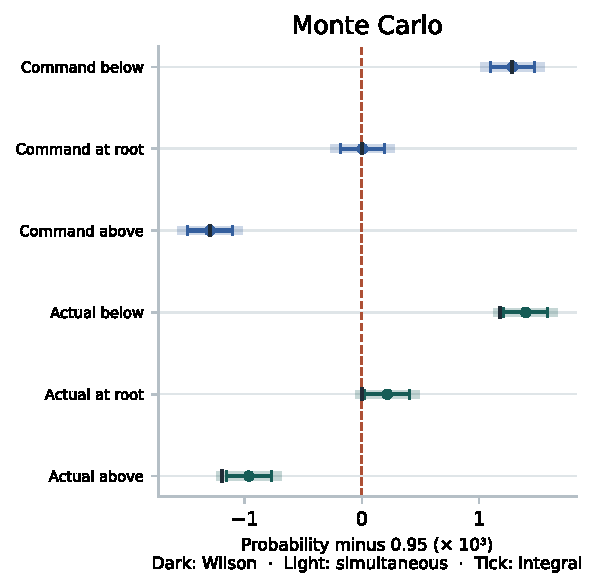
\includegraphics[width=0.55\linewidth]{figures/Q3-Monte-Carlo-Thresholds.pdf}
    \caption{Simulated coverage relative to the 95\% requirement at each travel limit and \(0.50\,\mathrm m\) below and above it. Dark bars show pointwise Wilson intervals and light bars show 95\% simultaneous intervals across all ten test points. Vertical ticks mark the integral estimates.}
    \label{fig:q3-test-mc}
\end{figure}

Fig.~\ref{fig:q3-parameters-80m} plots the parameter bounds in Eq.~(\ref{eq:q3-parameter-domain}). Holding \(b=0.02\,\mathrm{m/m}\) gives upper bounds on \(a\) of \(0.178721\,\mathrm m\) for commanded bearing and \(0.036745\,\mathrm m\) for actual pointing. At whole-centimeter resolution, the travel limits in Table~\ref{tab:q3-limits} round down to \(73.93\,\mathrm m\) and \(66.83\,\mathrm m\), respectively.

% 图与边界数据见 results/q3/80米参数域与误差贡献_蓝灰配色图集_20261121/。
\begin{figure}[!htbp]
    \centering
    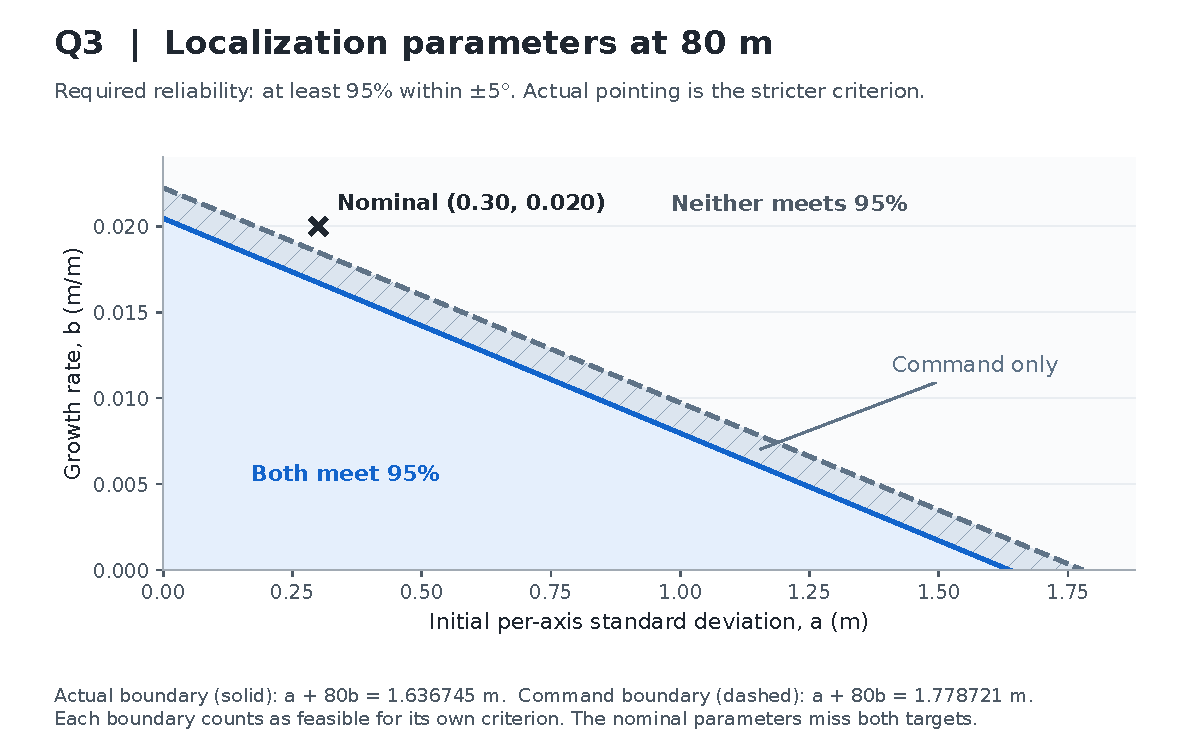
\includegraphics[width=0.9\linewidth]{figures/Q3-Parameters-at-80m.pdf}
    \caption{Localization parameters that meet the 95\% requirement after 80 m of travel at a horizontal target range of 40 m. Each criterion includes its boundary.}
    \label{fig:q3-parameters-80m}
\end{figure}

% 响应曲线、联合扰动及独立积分误差见 results/q3/测向参数敏感性与联合情景_20261122/。
Fig.~\ref{fig:q3-sensitivity} reports the changes in the actual-pointing travel limit and coverage at \(80\,\mathrm m\) under individual perturbations. The joint cases in Table~\ref{tab:q3-joint-sensitivity} apply all specified changes simultaneously. Gaussian half-plane integration confirmed the threshold classifications of all 66 evaluations and agreed with the projected-normal travel limits to within \(1.3\times10^{-10}\,\mathrm m\). Across these settings, the first-order normal approximation overestimated the travel limits by \(0.065\)--\(0.141\,\mathrm m\) and agreed on whether the coverage requirement was met at \(80\,\mathrm m\).

\begin{figure}[!htbp]
    \centering
    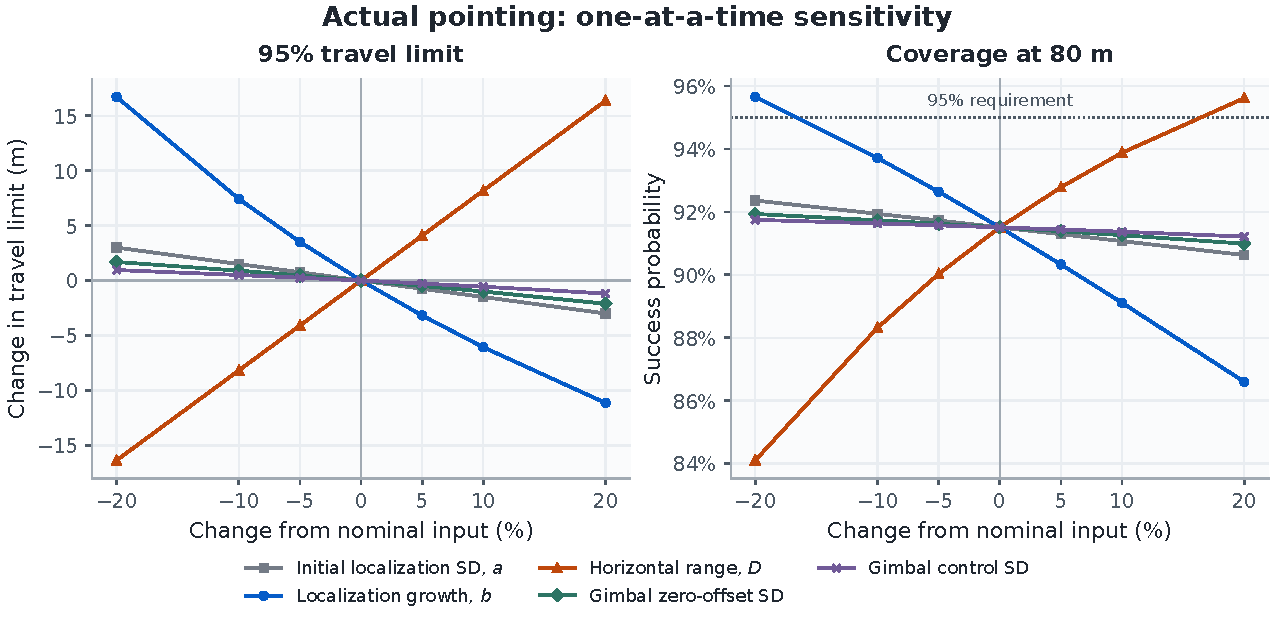
\includegraphics[width=\linewidth]{figures/Sensitivity-Q3.pdf}
    \caption{Changes in the travel limit at \(95\%\) coverage (left) and coverage probabilities at \(80\,\mathrm m\) (right) for actual pointing under individual parameter perturbations.}
    \label{fig:q3-sensitivity}
\end{figure}

\begin{table}[!htbp]
    \centering
    \caption{Travel limits at \(95\%\) coverage and coverage probabilities after \(80\,\mathrm m\) of cumulative travel.}
    \label{tab:q3-joint-sensitivity}
    \begin{tabular}{@{}lrrrr@{}}
        \toprule
        & \multicolumn{2}{c}{Commanded bearing} & \multicolumn{2}{c}{Actual pointing} \\
        \cmidrule(lr){2-3}\cmidrule(l){4-5}
        Setting & Limit (m) & \shortstack[r]{Coverage\\at 80 m} & Limit (m) & \shortstack[r]{Coverage\\at 80 m} \\
        \midrule
        Nominal & 73.936 & 93.347\% & 66.837 & 91.507\% \\
        Error parameters \(-10\%\), \(D\) \(+10\%\) & 93.700 & 97.508\% & 86.730 & 96.247\% \\
        Error parameters \(+10\%\), \(D\) \(-10\%\) & 57.766 & 86.671\% & 50.672 & 84.602\% \\
        \bottomrule
    \end{tabular}
\end{table}

% 排完 B.4 的响应图和联合工况表，再开始下一小节。
\clearpage

% 配对结果：results/q4/同毫米初排分区与全场配对_20261122/paired_cases.csv、paired_summary.csv。
% 分区实现：explore/b-first-round@30d54fa，src/q4/reschedule.py；适配见 checks/q4_paired_panel.py。
\subsubsection*{B.5 Local-Region Rescheduling and Policy Controls}
\label{app:q4-alternatives}

Local-Region Rescheduling (LR) builds a separate set of stations for each vehicle. Each set takes a \(4\times4\) grid in the vehicle's rectangle and includes its initial station, its in-region nominal stations and its position at dispatch. The rectangles, in meters and in vehicle order, are
\begin{equation}
\label{eq:q4-local-search-rectangles}
\begin{gathered}
\relax[2,32]\times[2,32],\qquad [66,98]\times[1.5,20],\qquad [2,30]\times[77.6,98],\\
\relax[81,98]\times[48,85],\qquad [36,67]\times[80,98].
\end{gathered}
\end{equation}
In the matched replay, field-edge sites are clipped to the inset boundary for \(0.45\,\mathrm m\) of body clearance. Transfers use feasible straight segments. A vehicle that keeps the same station and target completes any remaining slew. A vehicle that changes assignment first resets if its gimbal has not reached the travel attitude. For each pending alert and healthy pair, LR keeps the station pair with the earliest joint readiness. Each search layer adds an alert, updates vehicle stations and release times and retains up to 36 distinct states. States rank by latest start and then by the sum of release times. The best result at the deepest layer replaces the original queue if it improves the strict-retention score. The matched replay verifies the choice under the common prefix, lock and feasibility rules of Section~\ref{sec:q4-model}. The implementation returns the original queue when a healthy vehicle's dispatch position falls outside its assigned rectangle.

Fixed stations (FS) uses the field-wide search while keeping the two original stations for each pending old alert. It may change vehicles and service order. Retain and append (RA) preserves the original queue and attempts to add \(T_4\) once the selected vehicles are free of their original commitments and communication is available. Table~\ref{tab:q4-alternatives} summarizes the matched results. The mean uses the prescribed \(60\,\mathrm s\) score for any scenario in which an alert misses the window.

\begin{table}[!htbp]
    \centering
    \caption{Matched policy results. The two count columns give the number of scenarios with all alerts started or with five uninterrupted seconds of joint recording for every alert.}
    \label{tab:q4-alternatives}
    \setlength{\tabcolsep}{4pt}
    \begin{tabular}{@{}llrrr@{}}
        \toprule
        Rule & Policy & All start & \shortstack[r]{Complete\\recordings} & \shortstack[r]{Mean\\\(t_{\rm last}\) (s)} \\
        \midrule
        Main (1,751) & SR & 7 & 3 & 59.802 \\
                    & RA & 583 & 291 & 47.835 \\
                    & FS & 1,751 & 1,021 & 34.310 \\
                    & LR & 1,751 & 1,167 & 25.136 \\
                    & FW & 1,751 & 1,167 & 24.746 \\
        \addlinespace
        Joint restriction (1,314) & SR & 6 & 3 & 59.830 \\
                                & RA & 438 & 219 & 50.663 \\
                                & FS & 1,236 & 730 & 39.892 \\
                                & LR & 1,314 & 876 & 32.677 \\
                                & FW & 1,314 & 876 & 32.301 \\
        \bottomrule
    \end{tabular}
\end{table}

Both methods started every alert in all 1,751 main-rule scenarios. The mean \(t_{\mathrm{last}}\) was \(24.746\,\mathrm s\) for FW and \(25.136\,\mathrm s\) for LR. FW reached the last start earlier in 724 scenarios, tied in 1,024 and was later in three.

Table~\ref{tab:q4-matched-outage} pairs LR and FW on the same 1,314 outage scenarios under the main rule and the joint restriction. The two single restrictions in Table~\ref{tab:q4-outage-sensitivity} were evaluated for FW only. Imposing both restrictions increased the mean \(t_{\mathrm{last}}\) for LR by \(5.830\,\mathrm s\). Under each of the two paired rules, both methods achieved \(\eta=1\) in every outage scenario and completed five uninterrupted seconds of joint recording for every alert in 876 scenarios.

% 主规则配对按同目录 scenario_manifest.csv 的 t_rec_s 筛选含断联场景，逐场比较使用原验收器的 1e-8 s 同分容差。
\begin{table}[!htbp]
    \centering
    \caption{Mean \(t_{\mathrm{last}}\) and paired counts over 1,314 matched outage scenarios under the main rule and the joint restriction. The counts show whether FW's latest start was earlier than, tied with, or later than LR's.}
    \label{tab:q4-matched-outage}
    \begin{tabular}{@{}lrrrrr@{}}
        \toprule
        Rule & LR mean (s) & FW mean (s) & Earlier & Tied & Later \\
        \midrule
        Main rule, outage subset & 26.847 & 26.436 & 538 & 776 & 0 \\
        Both restrictions & 32.677 & 32.301 & 576 & 726 & 12 \\
        \bottomrule
    \end{tabular}
\end{table}

In Case~08, FW starts \(T_4\) \(0.118\,\mathrm s\) earlier than LR. Its \(V_5\) then drives for \(0.155\,\mathrm s\) to the \(T_3\) station, while LR holds \(V_5\) at the same station for both alerts. Since \(V_5\) determines the \(T_3\) start, FW reaches the last start \(0.049\,\mathrm s\) later.

In Case~10, FS replaces the failed \(V_2\) by sending \(V_4\) from its \(T_2\) station to the former \(V_2\) station. The \(60.901\,\mathrm m\) drive and subsequent slew give a joint start of \(43.965896\,\mathrm s\), compared with \(12.765521\,\mathrm s\) for FW and LR using \(V_5\) at its current position. In Case~11, all original alerts are locked at recovery. FW and RA choose a \(T_4\) station for \(V_3\) with a \(1.168\,\mathrm s\) drive, compared with \(3.336\,\mathrm s\) in LR. The \(T_4\) starts are \(23.836399\,\mathrm s\) for FW and RA and \(26.120941\,\mathrm s\) for LR. \hyperref[app:q4]{Appendix~A} records the assignments and events in these cases.

\clearpage
% OpenCode（Magpie, group/gpt-6.2-sol）于 2026-11-23 辅助复核附录 C 的底表、计算指向概率并拟订英文稿，供 AI 使用报告记录。
\subsection*{Appendix C. Verification of Scheduling and Pointing Results}
\label{app:verification}
\addcontentsline{toc}{subsection}{Appendix C. Verification of Scheduling and Pointing Results}

% 连续下界与剖分计数：results/q2/等精度快速部署与并发排程_20261121/continuous_bound.json。
% 全精度与毫米方案：results/q2/毫米部署与初排_全程净空四十五厘米_20261121/q22_refinement.csv。
\subsubsection*{C.1 Continuous-Domain Scheduling Bound}
\label{app:q22-bound}

Six observation slots and five vehicles force at least one reuse in Section~\ref{sec:q22-model}. The reused vehicle's first two alerts define one of 30 chains \(V_i:T_m\to T_n\). Let \(X,Y\) be station rectangles, \(d\) the Euclidean set distance and \(\underline{\tau}_j(X)\) a slew-time lower bound on \(X\) for \(T_j\). Let \(u_{-i,m}\) be the smallest readiness lower bound for \(T_m\) among the other four vehicles. With initial center \(p_i^0\) and speed \(v\), the second joint start is bounded below by
\begin{equation}
\label{eq:q22-continuous-bound}
\begin{aligned}
\underline{S}_{imn}(X,Y)={}&\max\!\left\{\frac{d(p_i^0,X)}{v}+\underline{\tau}_m(X),\ u_{-i,m}\right\}\\
&+5\,\mathrm s+\underline{\tau}_m(X)+\frac{d(X,Y)}{v}+\underline{\tau}_n(Y).
\end{aligned}
\end{equation}
The set distances bound route lengths from below. The first slew and its reset share the same lower bound.

The check subdivides the vehicle-center domain with body-clearance and pairing constraints relaxed. Visibility filtering discards rectangles wholly inside a building shadow with a \(10^{-8}\,\mathrm m\) allowance. A rectangle pair is discarded when its bound exceeds the trial by more than \(10^{-8}\,\mathrm s\). At \(10.352100\,\mathrm s\), the readiness and slew screen excludes 24 chains. Table~\ref{tab:q22-bound-chains} gives the remaining transfer-distance checks.

\begin{center}
    \begin{minipage}{\linewidth}
    \centering
    \captionsetup{type=table}
    \caption{Rectangle-pair evaluations after the initial screen, by vehicle and alert order.}
    \label{tab:q22-bound-chains}
    \setlength{\tabcolsep}{4pt}
    \begin{tabular}{@{}lrrrrrr@{}}
        \toprule
        Vehicle & \(T_1\to T_2\) & \(T_1\to T_3\) & \(T_2\to T_1\) & \(T_2\to T_3\) & \(T_3\to T_1\) & \(T_3\to T_2\) \\
        \midrule
        \(V_1\) & 0 & 0 & 0 & 0 & 135 & 0 \\
        \(V_2\) & 0 & 0 & 0 & 0 & 0 & 0 \\
        \(V_3\) & 352 & 2,230,398 & 0 & 0 & 329 & 0 \\
        \(V_4\) & 0 & 0 & 0 & 0 & 0 & 0 \\
        \(V_5\) & 43 & 385 & 0 & 0 & 0 & 0 \\
        \bottomrule
    \end{tabular}
    \end{minipage}
\end{center}

All 30 chains are excluded at the trial. The feasible full-precision schedule gives an upper bound of \(10.352118514\,\mathrm s\), leaving an interval \(18.514\,\mu\mathrm s\) wide. The millimeter plan in Table~\ref{tab:q22-millimeter} gives \(10.391510\,\mathrm s\). Run the check from the supporting archive root.

\begin{lstlisting}[language=bash]
nohup python3 -B -m checks.q2_continuous_bound \
  --trial-s 10.352100 --t1-partner-s 1.53203
\end{lstlisting}

\clearpage
% 比分与时序：results/q4/同毫米初排分区与全场配对_20261122/paired_cases.csv、run_record.md；提交包 S4/panel/。
\subsubsection*{C.2 Largest FW Delay Relative to LR}
\label{app:q4-delay}

In the joint-restriction sample, FW trails LR by up to \(0.113\,\mathrm s\) in \(t_{\rm last}\). This delay occurs at each sampled recovery time when \(T_4=(285^\circ,30\,\mathrm m,50\,\mathrm m)\) and \(V_1\) fails. Table~\ref{tab:q4-delay} shows the replay with recovery at 30 s. Both policies start every alert, and \(T_2\) is last.

\begin{center}
    \begin{minipage}{\linewidth}
    \centering
    \captionsetup{type=table}
    \caption{Critical events of \(V_3\) in scenario \texttt{E7\_A285\_R30\_V1\_C30} under both outage restrictions. Times are in seconds.}
    \label{tab:q4-delay}
    \setlength{\tabcolsep}{4pt}
    \begin{tabular}{@{}lrrrr@{}}
        \toprule
        Policy & \(T_4\) start & \(T_4\) reset ends & Arrival at \(T_2\) station & \(T_2\) start \\
        \midrule
        FW & 32.794768 & 39.743378 & 39.929717 & 43.523460 \\
        LR & 32.794768 & 39.756479 & 39.756479 & 43.410356 \\
        \bottomrule
    \end{tabular}
    \end{minipage}
\end{center}

LR uses the same station for both alerts on the \(V_3\) chain. FW moves \(V_3\) between stations after the \(T_4\) reset. FW spends \(0.186339\,\mathrm s\) driving and saves \(0.073236\,\mathrm s\) in reset and slew. Vehicle \(V_4\) is already ready for \(T_2\) in both policies, so the difference in \(V_3\)'s readiness determines the difference in \(t_{\rm last}\).

% 指向阈值：results/q3/测向可靠性与80米定位约束_五方法对照_20261120/reference_check.json。
% S4/panel/scenario_manifest.csv 给告警位置，alert_assignments.csv.gz 给站位与开测，vehicle_timelines.csv.gz 给开测前路径。
\subsubsection*{C.3 Pointing Coverage at New-Alert Stations}
\label{app:q4-pointing}

For each \(T_4\) vehicle in S4, let \(s_i\) be the sum of recorded travel segment lengths through the joint start and \(D_i\) the horizontal range from its archived station to the target. Table~\ref{tab:q4-pointing-coverage} counts scenarios where both vehicles meet the individual 95\% actual-pointing criterion from Section~\ref{sec:q3-model},
\begin{equation}
\label{eq:q4-new-station-coverage}
0.30\,\mathrm m+0.02s_i\ \le\ \sigma_{*,\mathrm{act}}(40\,\mathrm m)\frac{D_i}{40\,\mathrm m},
\qquad \sigma_{*,\mathrm{act}}(40\,\mathrm m)\simeq 1.636745169\,\mathrm m.
\end{equation}
\begin{center}
    \begin{minipage}{\linewidth}
    \centering
    \captionsetup{type=table}
    \caption{Scenarios with \(T_4\) in which both assigned vehicles individually reach 95\% modeled actual-pointing coverage.}
    \label{tab:q4-pointing-coverage}
    \setlength{\tabcolsep}{5pt}
    \begin{tabular}{@{}lrr@{}}
        \toprule
        Rule & FW & LR \\
        \midrule
        Main & 1,669 / 1,728 & 1,682 / 1,728 \\
        Both restrictions & 1,269 / 1,296 & 1,263 / 1,296 \\
        \bottomrule
    \end{tabular}
    \end{minipage}
\end{center}

In Case~12R of Table~\ref{tab:q4-representative-scores}, FW reaches the last start \(1.387\,\mathrm s\) earlier than LR. At the \(T_4\) start, \(V_3\) has traveled \(10.167\,\mathrm m\) in FW and \(14.699\,\mathrm m\) in LR. Its target range is \(8.464\,\mathrm m\) in FW and \(13.071\,\mathrm m\) in LR. The shorter range in FW gives a smaller ratio \(D_i/\sigma(s_i)\), and the individual pointing coverage is \(84.04\%\) in FW and \(92.67\%\) in LR. The other vehicle, \(V_4\), uses the same station and has coverage above \(99.99\%\) under both policies.

\clearpage
% 代码取自队员确认的支撑材料工作包，按其 README 的正文采用版核对。
% OpenCode（Magpie, group/gpt-6.2-sol）于 2026-11-23 辅助摘录、核对与排版，供 AI 使用报告记录。
\begingroup
\linespread{1}\selectfont
% 同一源码行折行后仍留在同一页，连续空行在 PDF 中合成一行。
\lstset{language=Python,
    basicstyle={\fontsize{10pt}{11pt}\selectfont\ttfamily\interlinepenalty=10000\relax},
    columns=fullflexible,keepspaces=true,breakindent=1em,emptylines=1,
    aboveskip=1.5mm,belowskip=1.5mm}

\subsection*{Appendix D. Key Python Code}
\label{app:reproduction}
\addcontentsline{toc}{subsection}{Appendix D. Key Python Code}

The file paths refer to the supporting archive \texttt{BSWBMCM2619567fj.zip}. Diagnostic messages in the excerpts are translated into English where needed.

\subsubsection*{D.1 Observable Region and Station Selection}

The feasibility masks test the field boundary, vehicle clearance, elevation and line of sight. The radial projection gives the selected station for the \(T_1\) scene in Section~\ref{sec:q1-model}.
The shadow is the convex hull of the footprint and its scaled projection. A point is blocked when it lies in every defining half-plane.

\noindent\path{peer_methods/experiments/b/q1_independent/solve.py}
\begin{lstlisting}
def shadow_hull(b):
    """Exact camera-plane projection of a closed prism, h_camera < h < H."""
    k = DZ / (HEIGHT - b["height"])
    corners = rectangle_corners(b)
    eight = np.vstack([corners, TARGET + k * (corners - TARGET)])
    hull = ConvexHull(eight)
    return k, eight[hull.vertices], hull.equations


def blocked_polygon(points, shadow, tol=0.0):
    """Halfspace test in the analytically projected convex shadow."""
    points = np.atleast_2d(points)
    equations = shadow[2]
    inside = np.ones(len(points), dtype=bool)
    for nx, ny, c in equations:
        inside &= nx * points[:, 0] + ny * points[:, 1] + c <= tol
    return inside


def masks(points, tol=0.0, oracle="polygon"):
    points = np.atleast_2d(points)
    field, obstacle = vehicle_geometry(points, tol)
    radius = np.linalg.norm(points - TARGET, axis=1)
    elevation = radius >= RMIN - tol
    blocked = np.zeros(len(points), dtype=bool)
    for b, shadow in zip(BUILDINGS, SHADOWS):
        if oracle == "polygon":
            blocked |= blocked_polygon(points, shadow, tol)
        else:
            blocked |= blocked_slab(points, b, tol_t=tol)
    return field, obstacle, elevation, ~blocked


def feasible(points, tol=0.0, oracle="polygon"):
    return np.logical_and.reduce(masks(points, tol, oracle))


def analytic_solution():
    phi_top = math.pi - math.asin((71 + RHO - TARGET[1]) / RMIN)
    phi_east = 2 * math.pi - math.acos((79 + RHO - TARGET[0]) / RMIN)
    ds = np.linalg.norm(VEHICLES - TARGET, axis=1)
    lower_bounds = np.abs(ds - RMIN)
    winner = int(np.argmin(lower_bounds))
    direction = (VEHICLES[winner] - TARGET) / ds[winner]
    point = TARGET + RMIN * direction
    return point, winner, lower_bounds, phi_top, phi_east
\end{lstlisting}

\subsubsection*{D.2 West--North Station Pair}

The west--north construction places both stations at the elevation-limited range. The bearing Jacobian gives the first-order position covariance in Section~\ref{sec:q21-model}.

\noindent\path{peer_methods/experiments/b/q2_analytic/solve.py}
\begin{lstlisting}
def solve_precision():
    t = TGT['T2']
    r = (t[2]-H0)/math.tan(math.radians(SCENE['elevation_deg'][1]))
    p, q = (t[0]-r,t[1]), (t[0],t[1]+r)
    legs = [make_leg(v,VEH[v],s,0.,'T2') for v,s in zip(('V3','V5'),(p,q))]
    assert max(l['travel_s'] for l in legs) <= SCENE['q2_1']['travel_limit_s']
    geo = geometry(p,q,'T2')
    normals = np.array([[-math.sin(angles(s,'T2')[0]), math.cos(angles(s,'T2')[0])] for s in (p,q)])
    jacobian = normals/np.array(geo['ranges_m'])[:,None]
    sigma = math.radians(SCENE['q2_1']['bearing_sd_deg'])
    cov = sigma**2 * np.linalg.inv(jacobian.T @ jacobian)
    for l in legs:
        l['vehicle_min_building_clearance_m'] = min(segment_clearance(*l['path'],b) for b in BLD.values())-R
    return dict(target='T2',target_xyz=t,legs=legs,**geo,covariance_m2=cov.tolist(),
                minimum_range_m=r,continuous_rmse_lb_m=sigma*math.sqrt(2)*r)
\end{lstlisting}

\subsubsection*{D.3 Concurrent Scheduling and Station Refinement}

The grid search prunes station pairs whose lower bound exceeds the incumbent. Sequential quadratic programming then refines the two stations of the reused vehicle in Section~\ref{sec:q22-model}.

\noindent\path{src/q2/schedule.py} (inside \texttt{search\_assignment})
\begin{lstlisting}[gobble=12]
            start = np.maximum(durations[0][:, None], durations[1])
            future = np.maximum(tail[target], np.maximum(remaining[0][:, None], remaining[1]))
            allowed = (start + future <= deadline) & self.problem.pair_mask(target, *site_ids)
            start[~allowed] = np.inf
            reused = [(target, v) in succ for v in vehicles]
            if all(reused):
                i, j = np.where(allowed)
            elif reused[0]:
                i, j = np.arange(start.shape[0]), np.argmin(start, axis=1)
            elif reused[1]:
                i, j = np.argmin(start, axis=0), np.arange(start.shape[1])
            else:
                row, col = np.unravel_index(np.argmin(start), start.shape)
                i, j = np.array([row]), np.array([col])
            bounds = (start + future)[i, j]
            for idx in np.argsort(bounds, kind="stable"):
                if bounds[idx] > self.best.latest_s + SELECT_TOL_S:
                    break
                a, b = i[idx], j[idx]
                starts[target] = float(start[a, b])
                selected[target] = ((vehicles[0], kept[0][a]), (vehicles[1], kept[1][b]))
                visit(depth + 1)
\end{lstlisting}

\noindent\path{src/q2/refinement.py}
\begin{lstlisting}
def _chain(scene, domains, reused, first, second, seeds, partner_ready, settings, decimals):
    first_domain, second_domain = domains[first], domains[second]
    home = scene.origins[reused]
    rounding = math.sqrt(2) * 0.5 * 10**-decimals if decimals is not None else 0.0
    buffer = settings["practical_station_gap_m"] + rounding if decimals is not None else 0.0
    los_gap = buffer + settings["nominal_visibility_gap_m"]
    wall = settings.get("wall_clearance_m", 0.0)
    wall_buffer = wall + rounding + 2 * PADDING_M if wall else 0.0
    first_ok, second_ok = (d.local_constraints(p, buffer, los_gap, wall_clearance_m=wall_buffer)
                           for d, p in zip((first_domain, second_domain), seeds))

    def limits(x):
        p, q, latest = x[:2], x[2:4], x[4]
        turn = first_domain.slew(p, scene.gimbal_deg_s)
        reused_ready = math.dist(home, p) / scene.speed_m_s + turn
        tail = scene.observation_s + turn + math.dist(p, q) / scene.speed_m_s
        tail += second_domain.slew(q, scene.gimbal_deg_s)
        return np.r_[latest - tail - partner_ready, latest - tail - reused_ready, first_ok(p), second_ok(q)]

    coordinates = np.ravel(seeds)
    radius = settings["search_radius_m"]
    fit = minimize(lambda x: x[-1], np.r_[coordinates, 12.0], method="SLSQP",
                   bounds=[*((x - radius, x + radius) for x in coordinates), (0, None)],
                   constraints={"type": "ineq", "fun": limits}, options={"ftol": 1e-12, "maxiter": 250})
    if not fit.success or limits(fit.x).min() < -1e-9:
        raise RuntimeError(f"Continuous refinement of the reuse chain failed ({fit.message})")
    sites = fit.x[:4].reshape(2, 2)
    return np.round(sites, decimals) if decimals is not None else sites
\end{lstlisting}

\subsubsection*{D.4 Bearing Reliability and Threshold}

Adaptive integration evaluates the projected-normal bearing density with the gimbal-error weight for actual pointing. Brent's method finds the localization standard deviation at the required coverage in Section~\ref{sec:q3-model}.

\noindent\path{src/q3/model.py}
\begin{lstlisting}
def projected_normal_angle_pdf(alpha_rad: float, sigma_m: float, range_m: float) -> float:
    if sigma_m <= 0.0:
        raise ValueError("Localization standard deviation must be positive for the density")
    kappa = range_m / sigma_m
    longitudinal = kappa * math.cos(alpha_rad)
    base = math.exp(-0.5 * kappa * kappa) / math.tau
    if longitudinal < 0.0:
        if base == 0.0:
            return 0.0
        c = -longitudinal
        return base * (1.0 - c * math.sqrt(math.pi / 2.0) * float(erfcx(c / math.sqrt(2.0))))
    transverse = kappa * math.sin(alpha_rad)
    return base + longitudinal / math.sqrt(math.tau) * math.exp(-0.5 * transverse * transverse) * float(ndtr(longitudinal))


def gimbal_success_probability_given_alpha(alpha_deg, threshold_deg: float, gimbal_deg: float,
                                           tail_tolerance: float = 1e-16):
    magnitude = np.abs(wrap180_deg(alpha_deg))
    if gimbal_deg == 0.0:
        return (magnitude <= threshold_deg).astype(float)

    def window(center):
        high = (threshold_deg - center) / gimbal_deg
        low = (-threshold_deg - center) / gimbal_deg
        return ndtr(high) - ndtr(low)

    periods, _ = wrap_window_count(threshold_deg, gimbal_deg, tail_tolerance)
    result = window(magnitude)
    for k in range(1, periods + 1):
        result = result + window(360.0 * k - magnitude) + window(360.0 * k + magnitude)
    return result


def _integrate_even(sigma_m: float, model: BearingModel, upper_rad: float, weight: Callable[[float], float],
                    tolerance: float, alternate: bool, extra_splits: tuple[float, ...] = ()) -> Integral:
    scales = (0.5, 2.0, 6.0, 13.0) if alternate else (1.0, 4.0, 12.0)
    breaks = [scale * sigma_m / model.range_m for scale in scales]
    interior = {point for point in (*breaks, math.pi / 2.0, *extra_splits) if 0.0 < point < upper_rad}
    edges = (0.0, *sorted(interior), upper_rad)
    segments = []
    for start, end in zip(edges, edges[1:]):
        width = end - start

        def integrand(t):
            angle = start + width * t
            pdf = projected_normal_angle_pdf(angle, sigma_m, model.range_m)
            return (2.0 * width * pdf) * weight(angle)

        outcome = quad(integrand, 0.0, 1.0, epsabs=tolerance / (len(edges) - 1),
                       epsrel=tolerance, full_output=True)
        if len(outcome) != 3:
            raise RuntimeError(f"Angular quadrature did not converge (sigma={sigma_m:g} m, [{start:g}, {end:g}] rad)\n{outcome[3]}")
        value, error, _ = outcome
        segments.append(AngleSegment(start, end, value, error))
    return Integral(math.fsum(seg.value for seg in segments),
                    math.fsum(seg.error for seg in segments), tuple(segments))


def reliability_1d_adaptive(sigma_m: float, model: BearingModel, mode: Mode,
                            tolerance: float = 2e-12, alternate: bool = False) -> Integral:
    gimbal = model.gimbal_sd_deg(mode)
    theta = model.threshold_deg
    if sigma_m < 0.0:
        raise ValueError("Localization standard deviation must be nonnegative")
    if sigma_m == 0.0:
        value = gimbal_success_probability_given_alpha(0.0, theta, gimbal, model.wrap_tail_tolerance)
        return Integral(float(value), 0.0)
    if gimbal == 0.0:
        result = _integrate_even(sigma_m, model, math.radians(theta), lambda _: 1.0, tolerance, alternate)
    else:
        def weight(angle):
            return float(gimbal_success_probability_given_alpha(
                math.degrees(angle), theta, gimbal, model.wrap_tail_tolerance,
            ))

        splits = tuple(math.radians(theta + k * gimbal) for k in (-3.0, 0.0, 3.0))
        result = _integrate_even(sigma_m, model, math.pi, weight, tolerance, alternate, splits)
    if not 0.0 <= result.value <= 1.0 + tolerance:
        raise RuntimeError(f"Integrated probability out of bounds ({result.value:g})")
    return replace(result, value=min(result.value, 1.0))


def solve_sigma_critical(probability: Callable[[float], float], minimum: float, start_m: float,
                         root_tolerance_m: float) -> float:
    at_zero = probability(0.0)
    if at_zero < minimum:
        raise ValueError("Gimbal error alone prevents the required coverage")
    if at_zero == minimum:
        return 0.0
    upper = start_m
    for _ in range(40):
        if probability(upper) < minimum:
            return brentq(lambda sigma: probability(sigma) - minimum, 0.0, upper, xtol=root_tolerance_m)
        upper *= 2.0
    raise RuntimeError("Failed to bracket the critical localization standard deviation")
\end{lstlisting}

\subsubsection*{D.5 Field-Wide Rescheduling}
\label{app:q4-search-settings}

At dispatch, joint starts strictly before the dispatch time are locked. The replayed phases determine each vehicle's position, gimbal pose and release time.

The shared station pool includes \(4\times4\) samples from each of five predefined rectangles. Each target's catalog draws on a filtered 1 m field grid, 0.25 m refinements around promising grid points and samples near the elevation limit. It retains sites from pairs with early joint readiness or low first-order RMSE (Section~\ref{sec:q21-model}). Post-dispatch stations are evaluated at their computed precision.

Both field-wide passes consider the eight earliest-ready stations per vehicle. For each vehicle pair, the first pass retains up to two station pairs and the second up to eight. If the shortlist yields no legal start within the window, the search checks the full available pool for that vehicle pair. Each layer keeps up to 36 distinct states and sends up to eight of them for replay. Restricted passes also supply candidates, including schedules that keep the original stations.

\noindent\path{src/q4/physics.py}
\begin{lstlisting}
def build_prefix(archive: Archive, failed: int | None, dispatch_s: float, *,
                 outage_rule: OutageRule | str = OutageRule.FULL_QUEUE) -> Prefix:
    if not DISTURBANCE_S <= dispatch_s <= 30 or (failed is not None and not 0 <= failed < len(archive.legs)):
        raise ValueError("Dispatch time or failed vehicle index is outside the problem bounds")
    rule = OutageRule(outage_rule)
    original, starts = _original_tracks(archive, failed, dispatch_s, rule)
    starts = dict(sorted(starts.items()))
    locked = {a: at for a, at in starts.items() if at < dispatch_s}
    states, fixed = [], []
    for v, phases in enumerate(original):
        phase = next(p for p in phases if p.start <= dispatch_s < p.end)
        if phase.kind == "OBSERVING" and phase.alert not in locked:
            phase = parking("READY_WAITING", dispatch_s, math.inf, phase.alert, phase.points[0], phase.pose0)
        if (rule.current_trip_only and phase.start == dispatch_s and phase.kind in {"TRAVELING", "SLEWING"}
                and any(row["target"] == archive.scene.targets[phase.alert] and row["depart_s"] >= DISTURBANCE_S
                        for row in archive.legs[v])):
            phase = parking("IDLE", dispatch_s, math.inf, None, phase.points[0])
        _, remaining = split_route(phase.points, (dispatch_s - phase.start) * archive.scene.speed_m_s)
        release = dispatch_s
        if phase.alert in locked and phase.kind in {"OBSERVING", "RESETTING"}:
            release = next(p.end for p in phases if p.alert == phase.alert and p.kind == "RESETTING")
        states.append(State(remaining[0], phase.pose(dispatch_s, archive.scene.gimbal_deg_s), phase.kind, phase.alert,
                            phase.end - dispatch_s if math.isfinite(phase.end) else None, remaining, release))
        fixed.append(_until(phases, release, archive.scene))
    return Prefix(failed, dispatch_s, locked, tuple(states), tuple(fixed), original, starts)
\end{lstlisting}

The beam search expands pending alerts from the replayed vehicle states, updating the assigned vehicles' release times. Finalists rank by the number of joint starts and the latest-start score. The continuous replay in \path{src/q4/recourse_experiment.py} checks them before selection in Section~\ref{sec:q4-model}.

\noindent\path{src/q4/recourse.py}
\begin{lstlisting}
def _beam(table, prefix, first, allowed, vehicles, settings, *, stations, alternatives):
    pending = tuple(a for a in range(len(table.pose)) if a not in prefix.locked)
    initial = Branch((), (-1,) * len(prefix.states), tuple(s.release for s in prefix.states), pending,
                     max(prefix.locked.values(), default=0.0), math.fsum(prefix.locked.values()))
    frontier = [initial]
    finalists = [initial]
    lim = settings["replay_candidates"]
    width = settings["beam_width"]
    counts = 0
    for _ in pending:
        children = []
        for node in frontier:
            for a in node.remaining:
                ready = np.array([first[v, a] if p < 0 else node.available[v] + table.distance_s[p] + table.slew[a]
                                  for v, p in enumerate(node.stations)])
                ready[~allowed[a]] = np.inf
                future = tuple(other for other in node.remaining if a != other)
                for v, w, p, q, start in _pairs(ready, table.pair_ok[a], vehicles, stations, alternatives):
                    last, release = list(node.stations), list(node.available)
                    last[v], last[w] = p, q
                    release[v] = start + table.scene.observation_s + float(table.slew[a, p])
                    release[w] = start + table.scene.observation_s + float(table.slew[a, q])
                    visit = Visit(a, v, w, p, q)
                    children.append(Branch((*node.visits, visit), tuple(last), tuple(release), future,
                                           max(node.latest, start), node.total + start))
        counts += len(children)
        frontier, seen = [], set()
        for node in sorted(children, key=Branch.rank):
            key = node.remaining, node.stations, tuple(round(t, 9) for t in node.available)
            if key in seen:
                continue
            seen.add(key)
            frontier.append(node)
            if len(frontier) == width:
                break
        if not frontier:
            break
        finalists.extend(frontier[:lim])
    return finalists, counts
\end{lstlisting}

\noindent Finalist selection in \texttt{propose}
\begin{lstlisting}[gobble=4]
    def ordered(cases):
        pending = len(table.pose) - len(prefix.locked)
        unique = {branch.visits: branch for branch in cases}
        return sorted(unique.values(), key=lambda b: (-len(b.visits),
                      round(b.latest, 8) if len(b.visits) == pending else HORIZON_S,
                      round(b.total, 8), b.visits))

    fixed, fixed_counts = search(table.fixed_allowed)
    flexible, flexible_counts = search(True)
    return {"fixed_stations": (ordered(fixed), fixed_counts),
            "recourse": (ordered(flexible + fixed), flexible_counts)}
\end{lstlisting}
\endgroup

\end{document}
